\newcommand*{\TeXturedVERSION}{1.5.0} %% TeXtured 2025-08-06
%%%%%%%%%%%%%%%%%%%%%%%%%%%%%%%%%%%%%%%%%%%%%%%%%%%%%%%%%%%%%%%%%%%%%%%
%% NOTE: If you find any issues or have any suggestions, please open %%
%%       an Issue on GitHub: https://github.com/jdujava/TeXtured     %%
%%%%%%%%%%%%%%%%%%%%%%%%%%%%%%%%%%%%%%%%%%%%%%%%%%%%%%%%%%%%%%%%%%%%%%%

%% Enable built-in LaTeX support for PDF/A compliance (must be before `\documentclass`)
\DocumentMetadata{lang=en, pdfversion=1.7, pdfstandard=A-2u}
\input{preamble/pdfA-compliance/glyphtounicode}

%% NOTE: Choose the desirable page layout version (electronic vs print)
\documentclass[12pt,a4paper]{report}                      % single-side (electronic)
% \documentclass[12pt,a4paper,openright,twoside]{report}  % two-sided (for printing)

%% Set some toggle flags to control some of the document properties
%% Define some toggle flags

\newif\ifFANCY       %% whether to enable some more fancy stylistic choices
\newif\ifWIP         %% whether to enable debug commands, todos, etc.
\newif\ifEXTRAMARGIN %% whether WIP mode has extra right margin
\newif\ifCENSOR      %% whether to censor denoted passages

\FANCYtrue        %% by default, enable fancy features

% \FANCYfalse % disable some of the more fancy stylistic choices
%% NOTE: Comment out the following lines for the final version
\WIPtrue            % THIS IS A WORK-IN-PROGRESS VERSION
% \EXTRAMARGINtrue  % add extra right margin in WIP version (for notes/corrections)
% \LINKBOXESfalse   % disable reference/link boxes for faster compilations
\CENSORtrue         % THIS IS A CENSORED VERSION

%% Preamble - data, packages, macros, and more
%%% Preamble

%% Data about the document, like title, author, etc.
%% Thesis type: bachelor, master, doctoral
\newcommand*{\ThesisType}{master}

%% Thesis title (exactly as in the formal assignment)
\newcommand*{\ThesisTitle}{\TeXtured{} Manual}
%% Plaintext version for PDF metadata, uncomment if needed (defauls to \ThesisTitle)
\newcommand*{\ThesisTitlePlaintext}{TeXtured Manual \TeXturedVERSION}
%% Thesis title (if custom formatting is needed for the title page, defauls to \ThesisTitle)
\newcommand*{\ThesisTitleFront}{
    \ThesisTitle\\
    {\Huge\color{gray}\TeXturedVERSION}
}

%% Author of the thesis
\newcommand*{\ThesisAuthor}{\textcolor{red}{Author's Name}}
%% Plaintext version for PDF metadata, uncomment if needed (defauls to \ThesisAuthor)
\newcommand*{\ThesisAuthorPlaintext}{Author's Name}

%% Year when the thesis is submitted
\newcommand*{\YearSubmitted}{2025}
%% Year of the last revision, uncomment if it is different from \YearSubmitted
% \newcommand*{\YearRevision}{2025}

%% University
\newcommand*{\University}{Charles University}

%% Name of the department or institute, where the work was officially assigned
%% (according to the Organizational Structure of MFF UK in English,
%% or a full name of a department outside MFF)
\newcommand*{\Department}{\textcolor{red}{Name of the Department/Institute}}

%% Is it a Department (katedra), or an Institute (ústav)?
\newcommand*{\DeptType}{Institute}

%% Thesis supervisor: name, surname and titles
\newcommand*{\Supervisor}{\textcolor{red}{Name, Surname, and Titles}}
%% Thesis co-supervisor: name, surname and titles (uncomment if applicable)
% \newcommand*{\CoSupervisor}{Name, Surname, and Titles}

%% Supervisor's department/institute (again according to Organizational structure of MFF)
\newcommand*{\SupervisorsDepartment}{\textcolor{red}{Supervisor's Department/Institute}}

%% Study programme and specialization
\newcommand*{\StudyProgramme}{\textcolor{red}{Study Programme}}

%% Abstract (recommended length around 80-200 words; this is not a copy of your thesis assignment!)
\newcommand*{\Abstract}{%
    \textcolor{red}{Write abstract here.}
}

%% Subject (short description for PDF metadata)
\newcommand*{\Subject}{%
    Write subject here.
}

%% Keywords (about 3-7)
\newcommand*{\Keywords}{%
    \textcolor{red}{Manual, Demo, Draft, WIP}
}
%% Plaintext version for PDF metadata, uncomment if needed (defauls to \Keywords)
\newcommand*{\KeywordsPlaintext}{%
    Manual, Demo, Draft, WIP
}


%% DEBUG: various helper debug goodies
\input{preamble/debug/commands}
\input{preamble/debug/line-numbers}
\usepackage{silence} % filter out unwanted warnings

\WarningFilter{latex}{Marginpar on page} % ignore "Marginpar on page ___ moved"


%% Colors
%% Colors
\usepackage[rgb,table]{xcolor} % color facilities

%% TODO: slightly darker gray color for "optional" words
\definecolor{ChapterNumberColor}{gray}{0.88}
\definecolor{HeaderColor}{gray}{0.35}
\definecolor{HeaderRuleColor}{gray}{0.75}
\definecolor{UrlColor}{RGB}{255,127,100}
\definecolor{CiteColor}{RGB}{127,230,252}

\definecolor{Gray10}{gray}{0.1}
\definecolor{Gray20}{gray}{0.2}
\definecolor{Gray30}{gray}{0.3}
\definecolor{Gray40}{gray}{0.4}
\definecolor{Gray50}{gray}{0.5}
\definecolor{Gray60}{gray}{0.6}
\definecolor{Gray70}{gray}{0.7}
\definecolor{Gray80}{gray}{0.8}
\definecolor{Gray90}{gray}{0.9}

\definecolor{LightGrayFill}{gray}{0.97}


%% Typesetting, figures, tables, etc.
%%% Typesetting, figures, tables, etc.

\ifpdftex % only for pdfLaTeX
    \usepackage[T1]{fontenc} % better support for accented characters
\fi
\usepackage{lmodern}  % Latin Modern fonts
\usepackage{romanbar} % Roman numerals with bars, provides `\Romanbar{...}`

%% Commands for accessing extra Latin Modern fonts
%%     - `sbc` - sans bold condensed
%%     - `sfq` - sans extended
%% https://www.tug.org/pracjourn/2006-1/robertson/robertson.pdf
\NewDocumentCommand{\sbcseries}{}{\sffamily\fontseries{sbc}\selectfont}
\NewDocumentCommand{\sfefamily}{}{\fontfamily{lmssq}\selectfont}
\DeclareTextFontCommand{\textsbc}{\sbcseries}
\DeclareTextFontCommand{\textsfe}{\sfefamily}

%% use slanted shape for emphasis `\emph{...}`, and for nested emphasis use italics
\DeclareEmphSequence{\slshape,\itshape}

\usepackage{microtype}           % improve typography
\DisableLigatures[-]{family=tt*} % disable ligatures in typewriter font
\usepackage{parskip}             % no paragraph indentation
\usepackage{csquotes}            % context-sensitive quotation facilities

%% Enumerate/itemize environments
\usepackage{paralist}   % improved enumerate and itemize
\setdefaultleftmargin{1.87em}{1.7em}{1.5em}{1em}{1em}{1em}
\setdefaultitem{$\bullet$}{\textbullet}{\textasteriskcentered}{\textperiodcentered}
\setdefaultenum{\bfseries (1)}{\bfseries (a)}{\bfseries (i)}{A.}

%% Configuration of figures, tables, captions, ...

%% Use same numbering for figures, tables, and equations
\makeatletter
\let\c@figure\c@table
\let\c@equation\c@table
\makeatother

%%% Graphics
\usepackage{graphicx}   % embedding of pictures
\graphicspath{          % default paths to figures
    {./figures/}
    {./figures/Inkscape/}
    {./frontmatter/img/}
}
%% Macro for appending to the graphics path
\ExplSyntaxOn
\NewDocumentCommand{\appendtographicspath}{m}{
    \tl_if_exist:cF { Ginput@path } { \tl_new:c { Ginput@path } }
    \tl_gput_right:cn { Ginput@path } { #1 }
}
\ExplSyntaxOff

%%% Tables
\usepackage{adjustbox}      % center big tables
\usepackage{array}          % custom column types in tables
\usepackage{booktabs}       % improved horizontal lines in tables

%% Increase default vertical space between rows in tables (default is 1.0)
\renewcommand*{\arraystretch}{1.1}

\IfPackageAtLeastTF{xcolor}{2024-09-29}{}{
    %% HACK: `ninecolors` is needed for `tabularray`, but fails to load with rgb color
    %%       model (before 2024/09/29) -> see https://tex.stackexchange.com/a/614702
    \selectcolormodel{natural}  % temporarily switch to natural color model
    \usepackage{ninecolors}     % now we can load `ninecolors` package
    \selectcolormodel{rgb}      % switch back to RGB color model
}

\usepackage{tabularray}     % advanced LaTeX tables
\usepackage{codehigh}       % verbatim in tables (with `\fakeverb` macro)
\UseTblrLibrary{amsmath, booktabs, siunitx} % load libraries for `tabularray`


%% Does \centering automatically, provides side captions (`\fcapside`) and much more
%% Inspired by the M-21 Institute of Engineering Thermodynamics figure template
\usepackage{floatrow}
\floatsetup{ % for all floats
    footnoterule = none,
    footposition = bottom,
}
\floatsetup[figure]{
    capbesideposition = right,
    capbesidesep = quad,
}

%% If you want to position the caption above the figure, use the following
% \floatsetup[table]{
%     style = plaintop, % caption always above, no matter where \caption is called
% }

%% Set caption width to be the same as the table width
% \floatsetup[longtable]{LTcapwidth=table} % https://tex.stackexchange.com/a/345772/120853

\usepackage{caption}    % customizing captions in floating environments
\usepackage{subcaption}

% \DeclareCaptionLabelSeparator{slash}{~/~} % `␣/␣` between label and caption
\DeclareCaptionLabelSeparator{slash}{\hspace{0.25em}/\hspace{0.25em}} % `␣/␣` between label and caption
\captionsetup{
    format        = plain,  % no hanging indent
    indention     = 0.6em,  % but still slightly indent the caption
    % format        = hang,   % alternative: hanging indent
    font          = small,
    labelfont     = {sf,bf},
    labelsep      = slash,
    labelformat   = simple,
    tableposition = bottom,
    parskip       = .3\baselineskip plus 1pt,
}

\makeatletter
% Make this new length and indent, same length as regular caption indent:
\newlength{\floatfootruleindent}
\setlength{\floatfootruleindent}{\caption@indent}% Set the new length
% A bit hacky; introduce a rule underneath caption if \floatfoot is called:
\renewcommand*{\floatfootskip}{2pt\color{Gray50}\hspace{\floatfootruleindent}\hrulefill}%
\makeatother

\DeclareCaptionFont{ftfont}{%
    \scriptsize%
    \color{Gray60}%
    \sffamily\raggedleft%
}
\captionsetup[floatfoot]{
    footfont=ftfont, % https://tex.stackexchange.com/q/9547/120853
}

%%% You can change the justification of all side-captions here
% \captionsetup[capbesidefigure]{
%     % When using sidecaptions, the linewidth can be rather small and awkward breaks and
%     % many underfull hboxes occur. Therefore, raggedright.
%     justification=raggedright,
% }
%
% \captionsetup[subfigure]{%
%     labelformat=simple,% 'parens' uses parantheses, 'brace' just the right one
%     labelsep=slash,%
%     labelfont={sf,bf},%
%     list=off,% list=off removes subfigures from LoF
% }%
%
% \captionsetup[subtable]{%
%     labelformat=simple,% 'parens' uses parantheses, 'brace' just the right one
%     labelsep=slash,%
%     labelfont={sf,bf},%
%     list=off,% list=off removes subfigures from LoF
% }%

%% Change counter from Arabic number to letter:
\renewcommand*{\theContinuedFloat}{\alph{ContinuedFloat}}


%% Hyperlinks, PDF metadata
%% Hyperlinks, PDF metadata
\usepackage[allowmove]{url}
\usepackage{hyperref}   % clickable links and metadata
\usepackage{nameref}    % cross-referencing by name
\usepackage{bookmark}   % more control over PDF bookmarks

%% Fallbacks for PDF metadata commands
\ProvideExpandableDocumentCommand{\ThesisAuthorPlaintext}{}{\ThesisAuthor}
\ProvideExpandableDocumentCommand{\ThesisTitlePlaintext}{}{\ThesisTitle}
\ProvideExpandableDocumentCommand{\KeywordsPlaintext}{}{\Keywords}

\hypersetup{
    linktoc=all,         % whole entry in TOC is clickable link
    pdfborder={0 0 0},   % to disable borders/frames around links
    pdflinkmargin=1.0pt, % extra link area around the text box (default 1pt)
    citebordercolor=CiteColor,
    linkbordercolor=LinkColor,
    urlbordercolor=UrlColor,
    % PDF metadata
    pdfauthor=\ThesisAuthorPlaintext,
    pdftitle=\ThesisTitlePlaintext,
    pdfsubject=\Subject,
    pdfkeywords=\KeywordsPlaintext,
    pdfcreator={LaTeX with hyperref, and biblatex/biber},
    pdfdisplaydoctitle, % https://tex.stackexchange.com/a/435434/120853
}
\bookmarksetup{
    numbered, % include chapter/section numbers in PDF outline
    open, openlevel=1, % expand bookmarks to level 1 (chapters)
}


%% NOTE: look of references, hyperlinks, and citations is customized
%%       mainly in `preamble/hacks/custom-reference-boxes.tex`


%% Miscellaneous commands/macros
%%% Macros for math symbols

%% Punctuation in math mode
\newcommand*{\eqend}{\,.}
\newcommand*{\eqcomma}{\,,}

%% Equals in given dimension
\NewDocumentCommand{\eqdim}{O{} m}{
    \IfBlankTF{#1}
    {\mathrel{\overset{\mathcolor{black!70}{d\.=\.#2}}{\scalebox{2.8}[1]{\(=\)}}}}
    {\mathrel{\overset{\mathcolor{black!70}{#2}}{\scalebox{#1}[1]{\(=\)}}}}
}
%% Phantom with relation spacing
\NewDocumentCommand{\relphantom}{m}{\mathrel{\phantom{#1}}}
%% Continuation of expression to the next line
\NewDocumentCommand{\graytimes}{}{\mathcolor{gray}{\times}}

% %% (Optional) Automatically use \mathcolor in math mode
% \NewCommandCopy{\textcolorOrig}{\textcolor}
% \RenewDocumentCommand{\textcolor}{O{} m m}{%
%     \ifmmode%
%         \let\colorcmd\mathcolor%
%     \else%
%         \let\colorcmd\textcolorOrig%
%     \fi%
%     \IfBlankTF{#1}{\colorcmd{#2}{#3}}{\colorcmd[#1]{#2}{#3}}%
% }

%% Determinants (use normal position of superscript/subscript)
\AddToHook{cmd/det/after}{\nolimits} % functionally replaces the following 2 lines
% \NewCommandCopy{\olddet}{\det}
% \renewcommand*{\det}{\olddet\nolimits}
\DeclareMathOperator{\Det}{Det}

%% Misc math macros
\NewCommandCopy{\transpose}{\intercal}
\DeclareMathOperator{\vol}{vol}
\DeclareMathOperator{\sgn}{sgn}
\newcommand*{\Id}{\bm{1}}
\newcommand*{\const}{\mathrm{const.}}
\DeclareMathOperator{\Span}{Span}
\DeclareMathOperator{\diag}{diag}
\newcommand*{\bdry}{\partial}
\newcommand*{\disjunion}{\sqcup} % TODO: spacing too small sometimes (in subscripts)
\NewDocumentCommand{\inclusion}{s}{\IfBooleanTF{#1}{\hookleftarrow}{\hookrightarrow}}
\NewDocumentCommand{\surjection}{s}{\IfBooleanTF{#1}{\twoheadleftarrow}{\twoheadrightarrow}}
\NewDocumentCommand{\exchange}{O{\quad}}{\xleftrightarrow{#1}}

%% Imaginary unit and Euler's number
%% inspired by Niklas Beisert
\NewDocumentCommand{\I}{}{\mathring{\imath}}
\NewDocumentCommand{\E}{s}{\IfBooleanTF{#1}{\mathrm{e}}{\mathinner{\mathrm{e}}}}

%% Big O notation (\biggO for centered O)
\NewDocumentCommand{\bigO} {l m}{\fbraces#1{\lparen}{\rparen}                   {O} {#2}}
\NewDocumentCommand{\biggO}{l m}{\fbraces#1{\lparen}{\rparen}{\raisemath{-0.1ex}{O}}{#2}}

%%% Various fields and number sets
\newcommand*{\R}{\mathbb{R}}
\newcommand*{\Z}{\mathbb{Z}}
\let\C\relax % avoid clashes with babel accent command when additional languages are loaded
\newcommand*{\C}{\mathbb{C}}
\newcommand*{\F}{\mathbb{F}}
\newcommand*{\N}{\mathbb{N}}

%% Group/Representation Theory
\DeclareMathOperator{\Hom}{Hom}
\DeclareMathOperator{\Ker}{Ker}
\DeclareMathOperator{\End}{End}
\DeclareMathOperator{\Aut}{Aut}
\DeclareMathOperator{\gl}{\mathfrak{gl}}
\DeclareMathOperator{\GL}{\mathsf{GL}}
\let\sl\relax % override (anyway deprecated) `sl` command
\DeclareMathOperator{\sl}{\mathfrak{sl}}
\DeclareMathOperator{\SL}{\mathsf{SL}}
\DeclareMathOperator{\oo}{\mathfrak{o}}
\DeclareMathOperator{\OO}{\mathsf{O}}
\DeclareMathOperator{\so}{\mathfrak{so}}
\NewDocumentCommand{\SO}{s}{\operatorname{\IfBooleanTF{#1}{\widetilde{\mathsf{SO}}}{\mathsf{SO}}}}
\DeclareMathOperator{\ISO}{\mathsf{ISO}}
\DeclareMathOperator{\spin}{\mathfrak{spin}}
\DeclareMathOperator{\Spin}{\mathsf{Spin}}
\let\U\relax % avoid clashes with babel accent command when additional languages are loaded
\DeclareMathOperator{\U}{\mathsf{U}}
\DeclareMathOperator{\su}{\mathfrak{su}}
\DeclareMathOperator{\SU}{\mathsf{SU}}
\DeclareMathOperator{\Sp}{\mathsf{Sp}}
\newcommand*{\g}{\mathfrak{g}}
\newcommand*{\rankgroup}{\mathsf{r}}

%%% Differential Geometry

\DeclareMathOperator{\Sect}{Sect}
\NewDocumentCommand{\Tangent}{s e{_}}{\IfBooleanTF{#1}{\bm{T}^{*}\mspace{-2mu}}{\bm{T}}\IfValueT{#2}{_{\mspace{-2mu}#2}}}
\NewDocumentCommand{\TSect}{s e{^_}}{\IfBooleanTF{#1}{\mathcal{T}^{*}\mspace{-2mu}}{\mathcal{T}}\IfValueT{#2}{^{#2}}\IfValueT{#3}{_{\mspace{0mu}#3}}\mspace{-2mu}}
\NewDocumentCommand{\Lie}{}{\mathcal{L}}
\DeclarePairedDelimiterX{\Liebracket}[2]{\dblbracketleft}{\dblbracketright}{#1,#2}
% \DeclarePairedDelimiterX{\Liebracket}[2]{\lbrack}{\rbrack}{#1,#2}

\DeclareMathOperator{\Tor}{\mathsf{Tor}}
\NewDocumentCommand{\Riem}{O{}}{\IfBlankTF{#1}{\bm{R}}{\tens{\bm{R}}{#1}}}
\NewDocumentCommand{\Ric}{O{}}{\IfBlankTF{#1}{\bmrm{Ric}}{\tens{\bmrm{Ric}}{#1}}}
\NewDocumentCommand{\Rscalar}{}{\mathcal{R}}

%% Override `physics` package command `\dd` to optionally use bold `d`
\RenewDocumentCommand{\dd}{s O{} m}{
    \mathinner{
        \IfBooleanTF{#1}{\bm{\mathrm{d}}}{\mathrm{d}}^{\mspace{-1mu}#2}#3
    }
}
%% Bold differential
\NewCommandCopy{\dotunderaccent}{\d}
\RenewDocumentCommand{\d}{O{} m}{\TextOrMath{\dotunderaccent{#2}}{\dd*[#1]{#2}}}


%% Covariant derivative (with optional arguments for space tweaking)
\NewDocumentCommand{\cder}{s O{a} e{_}}{
    \IfBooleanT{#1}{\mspace{-2mu}} % use starred variant when more \cder after each other
    \bm{\nabla}
    \IfValueT{#3}{             % when subscript index is given
        _{                     % start subscript
            \mspace{-7mu}      % remove extra space after nabla
            \chphantom{#3}{#2} % print #3 with the width of #2
        }
    }
}
%% Coordinate derivative
\NewDocumentCommand{\del}{s}{\IfBooleanTF{#1}{\partial}{\bm{\partial}}}
\NewDocumentCommand{\fdel}{O{} m}{{\frac{\del #1}{\del #2}}}
\NewDocumentCommand{\Dv}{O{} m}{{\frac{\bmrm{D} #1}{\mathrm{d} #2}}}
\NewDocumentCommand{\Laplacian}{}{\triangle}
\NewDocumentCommand{\dAlembertian}{s}{
    \mathord{\raisemath{0.07ex}{
            \mspace{1.5mu}
            \IfBooleanTF{#1}{\square[0.35em][boxframe=0.05em]}{\square[][boxframe=0.06em]}
            \.\.
        }}
}
% \RenewDocumentCommand{\dAlembertian}{s}{\mathord{\raisemath{-0.05ex}{\oldsquare}}}

%%% Tweaking of math index positioning, spacing, etc.
%%% (also definitions of new arrows, etc.)

%% TODO: see if \cramped{...} could be used sometimes to make
%%       (inline) math prettier (to avoid weird line spacing weird)

%% Modify size of `\bigwedge`/`\bigodot` and the position of their superscripts
\NewDocumentCommand{\Ext}{e{^}}{
    \scalerel*{\bigwedge}{\xmathstrut[-0.1]{0.1}} % scale down the \bigwedge a bit
    \IfValueT{#1}{^{\mspace{-2mu}#1}} % shift possible superscript little bit to the left
}
\NewDocumentCommand{\Odot}{e{^}}{
    \scalerel*{\bigodot}{\xmathstrut[-0.1]{0.1}} % scale down the \bigodot a bit
    \IfValueT{#1}{^{\mspace{-0mu}#1}} % (do not) shift possible superscript little bit to the left
}

%% Exchange \epsilon and \varepsilon
\NewCommandCopy{\oldepsilon}{\epsilon}
\NewCommandCopy{\oldvarepsilon}{\varepsilon}
\renewcommand*{\epsilon}{\oldvarepsilon}
\renewcommand*{\varepsilon}{\oldepsilon}

%% Math version of `\raisebox` and `\scalebox`
\NewDocumentCommand{\raisemath}{m}{\mathpalette{\raisemathAux{#1}}}% \raisemath{<len>}{...}
\NewDocumentCommand{\raisemathAux}{mmm}{\raisebox{#1}{\(#2#3\)}}
\NewDocumentCommand{\scalemath}{m O{}}{\mathpalette{\scalemathAux{#1}[#2]}}% \scalemath{<factor>}{...}
\NewDocumentCommand{\scalemathAux}{m O{} mm}{\IfBlankTF{#2}{\scalebox{#1}{\(#3#4\)}}{\scalebox{#1}[#2]{\(#3#4\)}}}

%% Modify subscript position
\NewDocumentCommand{\lowerindex}{O{0pt} O{0pt} e{_^}}{
    \IfValueT{#3}{_{\raisemath{#1}{#3}}}
    \IfValueT{#4}{^{\raisemath{#2}{#4}}}
}

%% Modify superscript/subscript positions for some greek letters
\NewCommandCopy{\oldchi}{\chi}
\renewcommand*{\chi}{\oldchi\lowerindex[-1.5pt]}
\NewCommandCopy{\olddelta}{\delta}
\renewcommand*{\delta}{\olddelta\lowerindex[1pt][1.0pt]}
\newcommand*{\bmdelta}{\bm{\olddelta}\lowerindex[1pt][1.0pt]}
\newcommand*{\altdelta}{{\olddelta\xmathstrut[-0.2]{0.0}}}
\newcommand*{\altbmdelta}{{\bm{\olddelta}\xmathstrut[-0.2]{0.0}}}

%% Smaller \in, \notin, \subset, ...
%% https://tex.stackexchange.com/questions/34393/the-mysteries-of-mathpalette
\NewDocumentCommand{\smallermath}{O{0.05ex} O{0.85} m}{\raisemath{#1}{\scalemath{#2}{#3}}}
\newcommand*{\smallplus}  {\mathrel{\smallermath{+}}}
\newcommand*{\textplus}   {\ensuremath{\.\smallplus\.}}
\newcommand*{\smallin}    {\mathrel{\smallermath{\in}}}
\newcommand*{\smallnotin} {\mathrel{\smallermath{\notin}}}
\newcommand*{\smallsubset}{\mathrel{\smallermath{\subset}}}
\newcommand*{\smallotimes}{\mathbin{\smallermath[0ex]{\oldotimes}}}
% \newcommand*{\smallotimes}{\.\smallerrel{\oldotimes}\.}


%% Fix spacing of \left( .. \middle| .. \right)
\NewCommandCopy{\leftOrig}{\left}
\NewCommandCopy{\rightOrig}{\right}
\NewCommandCopy{\middleOrig}{\middle}
\renewcommand*{\left}{\mathopen{}\mathclose\bgroup\leftOrig}
\renewcommand*{\right}{\aftergroup\egroup\rightOrig}
\RenewDocumentCommand{\middle}{sm}{\IfBooleanTF{#1}{\.\middleOrig#2\.}{\mathrel{}\middleOrig#2\mathrel{}}}
\NewDocumentCommand{\innermiddle}{m}{\mathinner{}\middleOrig#1\mathinner{}}

%% Less space around \setminus (\mathord instead of \mathinner)
\DeclareMathSymbol{\setminus}{\mathord}{symbols}{"6E}

%% Redefine `\square` to Young tableaux
\usepackage{ytableau}           % Young Tableaux
\ytableausetup{centertableaux}
\NewCommandCopy{\oldsquare}{\square}
\NewCommandCopy{\oldotimes}{\otimes}
\RenewDocumentCommand{\square}{O{0.55em} O{} O{}}{%
    \IfBlankTF{#1}{\ytableausetup{boxsize=0.55em}}{\ytableausetup{boxsize=#1}}%
    \ytableausetup{aligntableaux=top, boxframe = normal, #2}%
    \operatorname{\ydiagram[#3]{1}}%
}
\NewDocumentCommand{\smallsquare}{O{0.35em}}{\square[#1]}

%% Sizeable bullet
\NewDocumentCommand{\sbullet}{O{0.5}}{%
    \mathbin{\ThisStyle{\vcenter{\hbox{\scalebox{#1}{\(\SavedStyle\bullet\)}}}}}
}
\NewDocumentCommand{\fdot}{}{\mathcolor{black!80}{\sbullet[0.65]}}
\NewDocumentCommand{\adot}{}{\sbullet[0.52]}
\NewDocumentCommand{\idot}{s}{\mathcolor{darkgray}{\IfBooleanTF{#1}{\.\sbullet[0.4]\.}{\sbullet[0.4]}}}

%% (abstract) index placeholders
\NewDocumentCommand{\aind}{}{\bullet}
\NewDocumentCommand{\dind}{}{\mathcolor{black!60}{\sbullet[1.2]}}
\NewDocumentCommand{\ind}{}{\mathcolor{lightgray}{\bullet}}

%% Argument placeholder
\newsavebox{\argumentbox}
\sbox{\argumentbox}{%
    \begin{tikzpicture}[baseline=-0.6ex]
        \node(char)[draw, shape=rectangle, dash=on 1.2pt off 1.05pt phase 0.5pt, dash expand off,
            inner ysep=2pt, inner xsep=2pt, minimum size=0.6em, rounded corners=2pt] {};
    \end{tikzpicture}%
}
\NewDocumentCommand{\argument}{o}{%
    \IfValueTF{#1}{% use #1 as a scaling factor, resizebox relative to the text size
        \scalebox{#1}{\resizebox{!}{0.58em}{\usebox{\argumentbox}}}
    }{% choose scaling factor based on display/text/script/scriptscript math style
        \mathchoice{\argument[1.0]}{\argument[1.0]}{\argument[0.7]}{\argument[0.6]}
    }%
}

%% Curly arrows
\tikzset{
    leadsto/.style={-{Stealth[length=0.6em,open,round]},decorate,decoration={snake,amplitude=0.20ex,segment length=0.5em,pre length=0.2em,post length=0.6em}},
    toleads/.style={{Stealth[length=0.6em,open,round]}-,decorate,decoration={snake,amplitude=0.20ex,segment length=0.5em,pre length=0.6em,post length=0.2em}},
    correspondsto/.style={{Stealth[length=0.6em,open,round]}-{Stealth[length=0.6em,open,round]},decorate,decoration={snake,amplitude=0.20ex,segment length=0.5em,pre length=0.7em,post length=0.7em}},
}
\NewDocumentCommand{\longleadsto}{s O{} O{}}{%
    \ensuremath{\mathrel{
            \tikz[baseline=-0.5ex, inner sep=0ex, font=\scriptsize]{
                \node[minimum width=2.15em, inner xsep=0.6em, align=center] (a){\hphantom{#2}\\[0ex]\hphantom{#3}};
                \IfBlankF{#2}{\node[inner sep=0.3ex, above=0.3ex, xshift=-0.1em] at (a){#2};}
                \IfBlankF{#3}{\node[inner sep=0.3ex, below=0.3ex, xshift=-0.1em] at (a){#3};}
                \IfBooleanTF{#1}
                {\draw[line width=0.6pt, toleads] (a.west) -- (a.east);}
                {\draw[line width=0.6pt, leadsto] (a.west) -- (a.east);}
            }
        }}%
}
%% https://tex.stackexchange.com/questions/170092/xleftrightarrows-command-in-tikz-with-arrows-matching-the-latex-font?rq=1
\NewDocumentCommand{\correspondsto}{O{}O{}}{%
    \ensuremath{\mathrel{
            \tikz[baseline=-0.5ex, inner sep=0ex, font=\scriptsize]{
                \node[minimum width=3.48em, inner xsep=0.8em, align=center] (a){\hphantom{#1}\\[0ex]\hphantom{#2}};
                \IfBlankF{#1}{\node[inner sep=0.3ex, above=0.3ex] at (a){#1};}
                \IfBlankF{#2}{\node[inner sep=0.3ex, below=0.3ex] at (a){#2};}
                \draw[line width=0.6pt, correspondsto] (a.west) -- (a.east);
            }
        }}%
}

%% Quotient macro
\NewDocumentCommand{\bigslant}{O{0.2}O{1.7}mm}{
    \left.\mspace{-1mu}\raisemath{#1em}{#3}
    \mspace{-#2mu} \middleOrig/ \mspace{-\fpeval{#2+1}mu}
    \raisemath{-#1em}{#4} \mspace{-\fpeval{5*#1}mu} \right.
}
% \NewDocumentCommand{\coset}{O{0.05} O{0.1} m m}{\bigslant[#1][#2]{#3}{#4}}
\NewDocumentCommand{\coset}{O{}O{} m m}{#3/#4}
\NewDocumentCommand{\gt}{}{\bigslant{\g}{\mathfrak{t}}}
\NewDocumentCommand{\gts}{}{\bigslant[0.15]{\scriptstyle\g}{\scriptstyle\mathfrak{t}}}
\NewDocumentCommand{\onehalf}{}{\mspace{-2mu}\bigslant[0.15]{\scriptscriptstyle 1 \mspace{-1.2mu}}{\scriptscriptstyle 2}}

%% Cancel macro
\definecolor{cancelgray}{gray}{0.85}
\tikzset{
    main node/.style={inner sep=0,outer sep=0},
    label node/.style={inner sep=0.3em,font=\tiny,overlay},
    strike out/.style={shorten <=-.2em,shorten >=-.2em,overlay,thick,double distance = 0em,line cap=round},
}
\NewDocumentCommand{\cancel}{O{cancelgray}mo}{%
    \tikz[baseline=(N.base)]{
        \node[main node](N){\(#2\)};
        \IfValueT{#3}{\node[label node, gray, anchor=south] at (N.north){#3};}
        \draw[strike out, #1]  (N.south west) -- (N.north east);
    }
}

%% Macros for - links to packages, and verbatim macros for LaTeX commands
%%            - verbatim macros for commands defined specifically by TeXtured

%% will also utilize styles defined in `/preamble/hacks/custom-reference-boxes.tex`
\usepackage{tcolorbox}
\tcbset{
    packagebox/.style ={bottom=0.20ex, fontupper=\ttfamily},
    filebox/.style ={colframe=black!70!cyan!35, colback=black!10!cyan!3, bottom=0.20ex, fontupper=\ttfamily},
    dirbox/.style ={colframe=black!80!cyan!40, colback=black!60!cyan!8, bottom=0.20ex, fontupper=\ttfamily},
    macrobox/.style ={colframe=black!15, colback=black!3, bottom=0.20ex, fontupper=\ttfamily},
    custommacrobox/.style ={colframe=black!25!green!25, colback=black!5!green!5, bottom=0.20ex, fontupper=\ttfamily},
}

\NewTCBox{\packagebox}{!O{}}{link,hrefbox,packagebox,#1}
\NewTCBox{\filebox}{!O{}}{link,filebox,#1}
\NewTCBox{\dirbox}{!O{}}{link,dirbox,#1}
\NewTCBox{\macrobox}{!O{}}{link,macrobox,#1}
\NewTCBox{\custommacrobox}{!O{}}{link,custommacrobox,#1}

\ifLINKBOXES\else
    \RenewDocumentCommand{\packagebox}{O{} m}{\texttt{#2}}
    \RenewDocumentCommand{\filebox}{O{} m}{\texttt{#2}}
    \RenewDocumentCommand{\dirbox}{O{} m}{\texttt{#2}}
    \RenewDocumentCommand{\macrobox}{O{} m}{\texttt{#2}}
    \RenewDocumentCommand{\custommacrobox}{O{} m}{\texttt{#2}}
\fi

\NewDocumentCommand{\package}{m}{%
    % \href{https://texdoc.org/pkg/#1}
    \hrefold{https://ctan.org/pkg/#1}{%
        \packagebox[right=0.1em]{#1\textsuperscript{\tiny\(\,\to\,\)\textsf{CTAN}}}%
    }%
}
\NewDocumentCommand{\fileTeXtured}{O{-0.9\baselineskip} m}{
    \marginpar{
        \vspace{#1}
        \hspace{-\marginparsep}%
        \llap{%
            \filebox{#2}%
        }%
    }
}
\NewDocumentCommand{\dirTeXtured}{O{-1.3\baselineskip} m}{
    \marginpar{
        \vspace{#1}
        \hspace{-\marginparsep}%
        \llap{%
            \dirbox{#2}%
        }%
    }
}

\NewDocumentCommand{\macro}{O{}v}{\macrobox[#1]{#2}}
\NewDocumentCommand{\fakemacro}{O{}m}{\macrobox[#1]{\fakeverb{#2}}}
\NewDocumentCommand{\custommacro}{O{}v}{\custommacrobox[#1]{#2}}
\NewDocumentCommand{\fakecustommacro}{O{}m}{\custommacrobox[#1]{\fakeverb{#2}}}

%%% TikZ, and other drawing packages

\usepackage{tikz}
\usetikzlibrary{
    fadings,
    arrows.meta,
    calc,
    cd,
    decorations.pathmorphing, decorations.markings,
    trees,
    fit, matrix,
}

%% Directory Tree Structure
\tikzset{
    dirtree/.style={ % http://www.texample.net/tikz/examples/filesystem-tree/
        draw=black!80!cyan!40, thick, rounded corners=0.2em,
        growth parent anchor=west,
        grow via three points={one child at (1.0,-0.78) and
            two children at (1.0,-0.78) and (1.0,-1.56)},
        edge from parent path={([xshift=1.2em]\tikzparentnode.south west) |- (\tikzchildnode.west)},
        every node/.style={text=black, anchor=west, inner sep=0.7ex, draw=black!70!cyan!35, fill=black!10!cyan!3, text depth=.25ex, execute at begin node=\vphantom{Aj}},
        directory/.style={draw=black!80!cyan!40, fill=black!60!cyan!8},
        font=\ttfamily,
    },
}

%%% Quiver macros (for https://q.uiver.app/ diagrams)
%% A TikZ style for curved arrows of a fixed height, due to AndréC.
\tikzset{curve/.style={settings={#1},to path={(\tikztostart)
    .. controls ($(\tikztostart)!\pv{pos}!(\tikztotarget)!\pv{height}!270:(\tikztotarget)$)
    and ($(\tikztostart)!1-\pv{pos}!(\tikztotarget)!\pv{height}!270:(\tikztotarget)$)
    .. (\tikztotarget)\tikztonodes}},
    settings/.code={\tikzset{quiver/.cd,#1}
        \def\pv##1{\pgfkeysvalueof{/tikz/quiver/##1}}},
    quiver/.cd,pos/.initial=0.35,height/.initial=0}

%% TikZ arrowhead/tail styles.
\tikzset{tail reversed/.code={\pgfsetarrowsstart{tikzcd to}}}
\tikzset{2tail/.code={\pgfsetarrowsstart{Implies[reversed]}}}
\tikzset{2tail reversed/.code={\pgfsetarrowsstart{Implies}}}
%% TikZ arrow styles.
\tikzset{no body/.style={/tikz/dash pattern=on 0 off 1mm}}

%% Custom equal sign style - https://tex.stackexchange.com/a/443023
\tikzset{
    double line with arrow/.style args={#1,#2}{decorate,decoration={
        markings,%
        mark=at position 0 with {
            \coordinate (ta-base-1) at (0,1.2pt);
            \coordinate (ta-base-2) at (0,-1.2pt);
        },
        mark=at position 1 with {
            \draw[#1] (ta-base-1) -- (0,1.2pt);
            \draw[#2] (ta-base-2) -- (0,-1.2pt);
        }
    }},
    Equal/.style args={#1}{-,double line with arrow={{-,#1},{-,#1}}},
}

%% Inkscape figures
%% https://mirrors.nic.cz/tex-archive/info/svg-inkscape/InkscapePDFLaTeX.pdf
%% this is (and a lot more) already implemented in `svg` package, but no reason to use it
%% TODO: disable this for ArXiv submission (probably just leaving SVGs out will work fine)
\usepackage{shellesc}
\usepackage{filemod}
\NewDocumentCommand{\exportInkscapeSVG}{O{./figures/Inkscape/} m}{%
    \filemodCmp{#1#2.pdf}{#1#2.svg}{}{% regenerate PDF+LaTeX code if SVG is newer
        \ShellEscape{#1inkscape-export-to-latex "#1#2"}% use `inkscape-export-to-latex` script in the same directory
    }%
}
%% the third argument is the name of the SVG file without the extension
\NewDocumentCommand{\includeInkscapeSVG}{O{0.8\linewidth} O{./figures/Inkscape/} m}{%
    \exportInkscapeSVG[#2]{#3}%
    \def\svgwidth{#1}% set the width of the figure
    \input{#2#3.pdf_tex}%
}


%% Layout of the document, formatting of chapters, sections, TOC, etc.
%%% Page dimensions
%% single-side (electronic) -> use `\documentclass[12pt,a4paper]{report}`
%% two-sided (for printing) -> use `\documentclass[12pt,a4paper,twoside,openright]{report}`
\usepackage{geometry} % flexible interface for adjusting page layout/dimensions
\makeatletter
\if@twoside%
    \setlength\Gm@bindingoffset{15mm} % binding offset for two-sided printing
\fi%
\makeatother
\geometry{
    width=145mm,
    height=250mm,
    hmarginratio=1:1,   % space ratio between left and right margins
    vmarginratio=3:4,   % space ratio between top and bottom margins
    includehead,        % include header in total height
    headheight=2.5em,   % height of the header (includes space below the rule)
    headsep=0mm,        % no extra space between header and text
    % showframe,          % for DEBUG: helper lines for adjusting layout
}
\ifWIP\ifEXTRAMARGIN
        \geometry{
            paperwidth=260mm,   % PDF will be wider
            paperheight=297mm,  % A4 paper height
            layoutwidth=210mm,  % Real A4 content area
            layoutheight=297mm,
            layoutoffset=0mm,   % Align A4 layout to left edge
            % showcrop,
        }
        \usepackage{pict2e}
        \AddToHook{shipout/background}{% add gray line indicating the usual paper size
            \color{black!10}\linethickness{0.4pt}
            \put(210mm,0){\line(0,-1){297mm}}
        }
    \fi\fi

%% try to make text on all pages have the same height (default for `twoside`)
\flushbottom

%% Page numbering style and counters for different parts of the document
\makeatletter
\NewDocumentCommand{\frontmatter}{}{     % the front matter
    \pagenumbering{arabic}               %   arabic page numbering from the very first page
    \setcounter{page}{1}                 %   ensure the document starts at page 1
    \gdef\thechapter{\@Alph\c@chapter}   %   uppercase roman chapter numbering
}
\NewDocumentCommand{\mainmatter}{}{      % the main matter
    \cleardoublepage                     %   start on the right page
    \setcounter{chapter}{0}              %   reset chapter counter
    \setcounter{section}{0}              %   reset section counter
    \gdef\thechapter{\@arabic\c@chapter} %   arabic chapter numbering
}
\NewDocumentCommand{\backmatter}{}{      % the back matter (continue with arabic page numbering)
    \bookmarksetup{startatroot}          %   reset bookmarks level (in case parts are used)
    %% BUG: following line does not work as expected (adds space too late)
    % \addtocontents{toc}{\vspace{2ex}}    %   add some space after last part in TOC
}
\makeatother

%%% Headers and footers, page styles
\usepackage{fancyhdr}       % custom headers and footers
% \usepackage{extramarks}     % extra marks for headers and footers

%% Disable `fancyhdr` warning: "\fancyhead's `E' option without twoside option is useless.
%%                               Please consider using the `twoside' option"
\makeatletter
\def\f@nch@fancyhf@Echeck#1{}
\makeatother

\newlength{\headerpadding}  % left/right padding of header
\setlength{\headerpadding}{2pt}
% \RenewDocumentCommand{\chaptermark}{m}{\markboth{\chaptername\ \thechapter.\ #1}{\chaptername\ \thechapter.\ #1}}
% \RenewDocumentCommand{\sectionmark}{m}{\markright{\thesection.\ #1}}

%% Style of the header rule and decorations
\tikzset{
    header rule/.style={HeaderRuleColor,line width=0.9},
    header decor left/.style={HeaderRuleColor,line width=1.0,{Diamond[open]}-,overlay},
    header decor right/.style={HeaderRuleColor,line width=1.0,-{Diamond[open]},overlay},
}

%% Default header style (includes a rule with decorations)
\fancypagestyle{header}{
    \renewcommand*{\headrule}{
        % \renewcommand*{\headrulewidth}{0.9pt}
        % \textcolor{HeaderRuleColor}{\rule[1em]{\headwidth}{\headrulewidth}}%
        \tikz[baseline=-1em]{
            \fill[header rule] (0, 0) rectangle (\headwidth, 0.9pt);
            \ifFANCY % add fancy decorations
                \draw[header decor right] (\headwidth,0.45pt) -- ++(7pt,0);
                \draw[header decor left] (-7pt,0.45pt) -- (0,0.45pt);
            \fi
        }
    }
    \fancyhead[LO]{\hspace{\headerpadding}\textcolor{HeaderColor}{\textsf{\nouppercase{\leftmark}}}}
    % \fancyhead[LO]{\hspace{\headerpadding}\textcolor{HeaderColor}{\textsf{\nouppercase{\rightmark}}}}
    \fancyhead[RE]{\textcolor{HeaderColor}{\textsf{\nouppercase{\rightmark}}}\hspace{\headerpadding}}
    \fancyhead[RO]{\textbf{\thepage}\hspace{\headerpadding}}
    \fancyhead[LE]{\hspace{\headerpadding}\textbf{\thepage}}
    \ifWIP % show draft watermark in footer
        \fancyfoot[C]{\vskip1ex\relax \ttfamily\textcolor{black!15}{Draft - \today}}
    \else
        \fancyfoot{}
    \fi
}
%% For chapter pages, the `plain` style is used
\fancypagestyle{plain}[header]{
    \renewcommand*{\headrule}{
        \hfill\tikz[baseline=-1em]{
            \fill[header rule, path fading=west] (0, 0) rectangle (0.45\headwidth, 0.9pt);
            \ifFANCY % add fancy decorations
                \draw[header decor right] (0.45\headwidth,0.4pt) -- ++(7pt,0);
            \fi
        }
    }
    \fancyhead[LO,RE]{}
}
\pagestyle{header} % set up default header style

%% Chapter without number, but included in header and TOC
\NewDocumentCommand{\chapternotnumbered}{m}{
    \chapter*{#1}
    \markboth{#1}{#1}                   % use chapter title in header
    \addcontentsline{toc}{chapter}{#1}  % include chapter in TOC
}

%%% Chapter and section formatting
%% `clearempty` option removes page numbers from empty pages when using `\cleardoublepage`
\usepackage[newparttoc, clearempty]{titlesec}

%% NOTE: also include `\phantomsection` so that hyperlink anchors are properly placed 
%%                                                     (even non-numbered subsections)
\titleformat{\section}   {\phantomsection\Large\sffamily\bfseries}{\thesection}   {0.8em}{}
\titleformat{\subsection}{\phantomsection\large\sffamily\bfseries}{\thesubsection}{0.8em}{}

%% Part title (page) formatting
\titleformat{\part}[display]
{\thispagestyle{empty}\sffamily}
{\LARGE Part \Romanbar{\thepart}}
{0.2em}{\fontsize{30pt}{36pt}\selectfont\bfseries}

%%% Chapter title formatting
%% No extra space above and below chapter headings, big number/letter behind chapter title
%% inspired by https://tex.stackexchange.com/a/690632
\NewDocumentCommand{\chaphead}{m O{}}{
    \vspace*{-25pt}% reduce vertical space before the title
    {\setlength{\parindent}{0pt}\raggedright
        \Huge\sffamily\bfseries
        \ifFANCY%
            \chapterheadingletter{#2}% fancy Chapter number/letter
        \else%
            \IfBlankF{#2}{\thechapter\hspace{0.7em}}% just basic Chapter number
        \fi%
        #1\par\nobreak% Chapter title
        \vspace{20pt}% extra vertical space after the title
    }
}
%% -> modifying /usr/share/texmf-dist/tex/latex/base/report.cls
\makeatletter
\def\@makechapterhead#1{\chaphead{#1}[\thechapter]} % For numbered Chapters use their number
\def\@makeschapterhead#1{
    \ifFANCY
        \chaphead{#1}[\extract{#1}{1}] % extract first letter of the current chapter title
    \else
        \chaphead{#1} % just Chapter title
    \fi
}
\makeatother

%% Chapter number/letter formatting
\NewDocumentCommand{\chapterheadingletter}{m}{%
    \makebox[0pt][l]{%              Make box of zero width, don't move other stuff horizontally
        \raisebox{-16pt}[0pt][0pt]{% Align the number vertically, don't move other stuff vertically
            \hspace{6pt} \color{ChapterNumberColor}% Horizontal whitespace, text color
            \usefont{T1}{qzc}{m}{it}\fontsize{95pt}{95pt}\selectfont% Font type and size (TeX Gyre Chorus)
            #1 % Chapter heading letter
        }%
    }%
}
%% Macro to extract first `#2` characters from `#1`
%% https://tex.stackexchange.com/questions/402835/extract-first-character-of-string-stored-in-macro-using-expl3
%% TODO: latex treesitter grammar support ExplSyntaxOn/Off, command names containting also `_:`
\ExplSyntaxOn
\cs_generate_variant:Nn \tl_item:nn { f }
\DeclareExpandableDocumentCommand{\extract}{mm}{
    \tl_item:fn { #1 } { #2 }
}
\ExplSyntaxOff

%% Table of Contents
% \addtocontents{toc}{\vspace{-0.9em}}  % change space after "Contents" title in TOC
\newcommand*{\contentsandlists}{
    {\hypersetup{hidelinks}
        \tableofcontents

        %% Add list of structured environments
        %%  -> see `keytheorems` package documentation for more customization
        % \newcommand*{\listtheoremname}{List of Definitions, Remarks, \ldots}
        % \cleardoublepage\MakeLinkTarget{}
        % \currentpdfbookmark{\listtheoremname}{loe} % add PDF Index/Outline entry
        % \listofkeytheorems[onlynamed, swapnumber, title=\listtheoremname]

        %% Add list of figures and tables
        %%  -> see `tocbibind` package (or maybe also `titletoc`)
        % \listoffigures
        % \listoftables
    }
}

%%% TOC formatting
\usepackage{titletoc}   % formatting of TOC entries
\usepackage{tocbibind}  % more things in table of contents

\setcounter{secnumdepth}{1} % subsections are not numbered (no need for *), but are included in the TOC
\setcounter{tocdepth}{2}    % include subsections in toc, but not subsubsections (this is the default)
\contentsmargin[0.6em]{2em} % margin for the page numbers in the TOC

%% bold math for chapter titles in TOC, slightly bigger space between label and title
%% BUG: pdfLaTeX with changed `\contentsmargin` does not properly align page numbers
%%             (works properly when using absolute \contentsmargin, or with luaLaTeX)
%% HACK: to obatain consistent placement of page numbers (bold or not), we need to toggle
%%       off `\bfseries` with `\normalfont`, and only then apply it inside `\contentspage`
\titlecontents{chapter}[1.6em]{\addvspace{2.4ex}\bfseries} % <section> <left> <above-code>
{\contentslabel{1.4em}}{\hspace*{-1.4em}} % <numbered-entry-format> <numberless-entry-format>
{\hfill\normalfont\contentspage[\bfseries\thecontentspage]} % <filler-page-format> <--- HACK

%% prettier visual alignment of section label with chapter title
\titlecontents{section}[4.0em]{} % <section> <left> <above-code>
{\contentslabel{2.3em}}{\hspace*{-2.3em}} % <numbered-entry-format> <numberless-entry-format>
{\textcolor{gray}{\titlerule*[9pt]{.}}\contentspage} % <filler-page-format>

%% subsection entries in TOC are "inline" separated by a bullet
\titlecontents*{subsection}[4.7em]{\footnotesize\color{Gray40}}  % <section> <left> <above-code>
{}{}{~\thecontentspage} % <numbered-entry-format> <numberless-entry-format> <filler-page-format>
[][\ \textbullet\ ][\hspace*{0.6em}\vspace{0.1em}]  % <begin> <separator> <end>

%% part entries in TOC are centered, bigger, and without page number
\titlecontents{part}[2em]{\addvspace{3ex}\filcenter} % centered part title
{\small \partname~\thecontentslabel\\*[-0.2ex]\Large\bfseries}{\Large\bfseries}
{}[\addvspace{1.0ex}] % without page number



%% Bibliography/References configuration
%%% References/Bibliography
\usepackage[
    style=ext-numeric-verb, sorting=none,
    date=year, articlein=false, isbn=false,
    maxnames=16, maxcitenames=4,
    backref=true, backrefstyle=none,
    datamodel=preamble/references/biblatex-extra-fields,
]{biblatex}

%% Custom bibliography fields can be added in `preamble/references/biblatex-extra-fields.dbx`
%% see for example explanation in https://suchicodes.com/resources/blog/65a59395

%% Add bibliography resource
\addbibresource{preamble/bibliography.bib}

\newcommand*{\references}{
    \defbibheading{bibintoclabel}[\bibname]{%
        \chapter*{##1}%
        \label{ch:References}%
        \addcontentsline{toc}{chapter}{##1}%
        \markboth{##1}{##1}%
    }
    \defbibnote{note}{%
        % \vspace{-3em}
        \begin{flushright}
            \footnotesize
            % Asterisk in [\textcolor{black!35}{Author(s) Year}*] and (\textcolor{black!35}{Year}*) marks a secondary source/review article. \\
            % Asterisk in \texttt{[\({\mspace{1mu}\color{black!30}\bullet}\)*]} marks a secondary source/review article. \\
            Back-references to the pages where the publication was cited are given by \pagebox{\(\color{black!60}\bullet\)}.
        \end{flushright}
        \vspace{0.4em}
    }
    % \emergencystretch=1em % prevent some of the overfull hboxes
    % \hyphenpenalty 100 % try to prevent (some) hyphenation
    % \printbibliography[heading=bibintoc, title=References]
    \printbibliography[heading=bibintoclabel, title=References, prenote=note]
}


%%% Custom categories
%% `todo` category for references to be added (marked with red)
\DeclareBibliographyCategory{todo}
\addtocategory{todo}{TODO}

%% `secondary` category for secondary sources (will be marked with `*`)
\DeclareBibliographyCategory{secondary}
%% add secondary citations to this category 
\addtocategory{secondary}{secondary_review}


%% Modification of fields
%%% Modification of fields in References/Bibliography

%% if DOI is present, remove URL
%% ignore certain fields completely
%% set year to current year if title is TODO
\DeclareSourcemap{
    \maps[datatype=bibtex]{
        \map[overwrite]{
            \step[fieldsource=doi, final]  % if DOI is not present, terminate
            \step[fieldset=url, null]      % (if DOI is present) remove URL
            % \step[fieldset=eprint, null]
        }
        \map{
            \step[fieldset=pages, null]
            \step[fieldset=number, null]
            \step[fieldset=volume, null]
            \step[fieldset=series, null]
            \step[fieldset=location, null]
            \step[fieldset=address, null]
        }
        \map{
            \step[fieldsource=title, match={TODO}, final] % match TODO in title
            \step[fieldset=year, fieldvalue={\the\year}]  % set year to current year
        }
    }
}

%% Custom localisation strings
\DeclareCapitalPunctuation{} % disable automatic capitalization of localisation strings
\NewBibliographyString{arxiv, github, gitlab} % define new localisation strings
\DefineBibliographyStrings{english}{
    url = {{}\textsc{url}},     % included `{}` to avoid automatic capitalization, see
    arxiv = {{}\textsc{arXiv}}, % https://tex.stackexchange.com/a/472547 for more details
    github = {\textsc{GitHub}},
    gitlab = {\textsc{GitLab}},
    in = {\footnotesize\textsc{In}},
    % in = {},
    editor = {editor},
    editors = {editors},
}

%% smaller space after "in:"
\renewcommand*{\intitlepunct}{{\footnotesize\addcolon\,}}
% \renewcommand*{\intitlepunct}{\addcolon\space}

%% TODO: PhD or Ph.D.?


%% Modification of `cite` command -> wrap whole citation with a `tcolorbox` frame
%%% Wrap whole citation with braces in a `\citebox` frame, the whole being clickable link

% \DeclareOuterCiteDelims{cite}{\bibopenbracket}{\bibclosebracket}
\DeclareOuterCiteDelims{cite}{}{} % disable default outer delimiters

%% modifying /usr/share/texmf-dist/tex/latex/biblatex/cbx/numeric-verb.cbx
%% loaded subsequently in /usr/share/texmf-dist/tex/latex/biblatex-ext/ext-numeric-verb.cbx
\renewbibmacro*{cite}{%
    \printtext[bibhyperref]{%
        \citebox{%    <---- wrap the whole citation with a `tcolorbox` frame
            %% turn postnote into custom prenote
            \iffieldundef{postnote}{}{{\normalfont\hspace{0.18em}\printfield{postnote}\hspace{0.15em}}}%
            \lbrack%  <---- always consistently use brackets
            \printfield{labelprefix}%
            \printfield{labelnumber}%
            \ifbool{bbx:subentry}{\printfield{entrysetcount}}{}%
            \rbrack%  <---- always consistently use brackets
        }%
    }%
}

%% do not put commas between multiple citations when using `\cite{something,something}`
\renewcommand*{\multicitedelim}{\space}
% \renewcommand*{\multicitedelim}{\addsemicolon\space}

%% disable default postnote
\renewbibmacro*{postnote}{%
    % \iffieldundef{postnote}
    % {}
    % {\setunit{\printdelim{postnotedelim}}%
    %     \printfield{postnote}}
}

%%% Alternative style of multicitations
% \renewcommand*{\multicitedelim}{\addcomma} % no space between multiple citations, just a comma
%
% %% wrap the citation commands in a `\citebox`
% \NewCommandCopy{\autociteOrig}{\autocite}
% \NewCommandCopy{\citeOrig}    {\cite}
% \RenewDocumentCommand{\autocite}{O{} O{} m}{\citebox{\autociteOrig[#1][#2]{#3}}}
% \RenewDocumentCommand{\cite}    {O{} O{} m}{\citebox{\citeOrig[#1][#2]{#3}}}


%% Style tweaks
%%% References style tweaks

%% separation modifications
\setlength\bibitemsep{0.53\baselineskip}
\setlength\biblabelsep{1.5\labelsep}

%% label number always in brackets with monospaced font
%% -> modifying /usr/share/texmf-dist/tex/latex/biblatex/bbx/numeric.bbx
\DeclareFieldFormat{labelnumberwidth}{\ttfamily\mkbibbrackets{#1}}
% \DeclareFieldFormat{labelnumberwidth}{\citebox{\mkbibbrackets{#1}}}

%% red color for `todo` category
%% asterisk in labelnumber for secondary sources (in `secondary` category)
\DeclareFieldFormat{labelnumber}{%
    \ifcategory{todo}{\color{red}\(\sbullet[1.2]\)}{#1}%
    \ifcategory{secondary}{*}{}%
}

%% names in "small caps"
% \DeclareNameWrapperFormat*{author}{\textsc{#1}}

%% type "editor(s)" in parentheses
\DeclareFieldFormat{editortype}{\mkbibparens{#1}}
\DeclareDelimFormat{editortypedelim}{\addspace}

%% titles in sans (with red for `todo` category)
\DeclareFieldFormat*{title}{\sffamily\ifcategory{todo}{\textcolor{red}{#1}}{#1}}

%% punctuation between title and subtitle
\renewcommand*{\subtitlepunct}{\space{\normalfont\textbullet}\space}

%% emphasize publishers (same as journals in IEEE style)
% \DeclareListFormat{publisher}{\mkbibemph{#1}}

%% emphasize journals and publishers, in dark gray color
% \DeclareListFormat{publisher}{\mkbibemph{\textcolor{darkgray}{#1}}}
% \DeclareFieldFormat{journaltitle}{\mkbibemph{\textcolor{darkgray}{#1}}}
% \DeclareFieldFormat{booktitle}{\mkbibemph{\textcolor{darkgray}{#1}}}

%% date in bold (without parentheses)
\DeclareFieldFormat{issuedate}{#1}
\renewcommand*{\volnumdatedelim}{\addcomma\space}
\DeclareFieldFormat*{date}{\mkbibbold{#1}}
% \DeclareFieldFormat*{date}{\ifcategory{secondary}{\mkbibbold{#1}*}{\mkbibbold{#1}}}
% \DeclareFieldFormat{biblabeldate}{\mkbibparens{\mkbibbold{#1}}}


%% Customize DOI/arXiv/GitHub/URL formatting
%% add format for `github`/`gitlab` field
\DeclareFieldFormat*{github}{%
    \bibstring{github}\addcolon\space%
    \ifhyperref{\href{https://github.com/#1}{\nolinkurl{#1}}}{\nolinkurl{#1}}%
}
\DeclareFieldFormat*{gitlab}{%
    \bibstring{gitlab}\addcolon\space%
    \ifhyperref{\href{https://gitlab.com/#1}{\nolinkurl{#1}}}{\nolinkurl{#1}}%
}

%% put DOI/arXiv/GitHub/URL on a new line
%% support also `github` field
%%  -> changed from /usr/share/texmf-dist/tex/latex/biblatex-ext/ext-standard.bbx
\renewbibmacro*{doi+eprint+url}{%
    \setlength{\parskip}{0pt} % fix spacing of \fullcite in the body text of the document
    \ifboolexpr{
        test {\iffieldundef{doi}} and
        test {\iffieldundef{url}} and
        test {\iffieldundef{eprint}} and
        test {\iffieldundef{github}} and
        test {\iffieldundef{gitlab}}
    }{}{\printtext{\par}} % doi+eprint+url are printed on a new line
    \footnotesize    % make it small, so it (ideally) fits on one line
    \raggedright     % right-align the text (so that there are no overfull hboxes for long URLs)
    \renewcommand{\newunitpunct}{\space}                  % no periods on this line
    \renewcommand{\newblockpunct}{\penalty-9\relax\space} % avoid line breaks after labels "DOI:", "arXiv:", ...
    \ifboolexpr{togl {bbx:doi} and not test {\iffieldxref{doi}}}{\printfield{doi}}{}%
    \newunit\newblock
    \ifboolexpr{togl {bbx:eprint} and not test {\iffieldxref{eprint}}}{\usebibmacro{eprint}}{}%
    \newunit\newblock
    \ifboolexpr{not test {\iffieldxref{github}}}{\printfield{github}}{}% <--- added print of `github` field
    \newunit\newblock
    \ifboolexpr{not test {\iffieldxref{gitlab}}}{\printfield{gitlab}}{}% <--- added print of `gitlab` field
    \newunit\newblock
    \ifboolexpr{togl {bbx:url} and not test {\iffieldxref{url}}}{\usebibmacro{url+urldate}}{}
}

%% print arXiv via \bibstring{arxiv}
%%  -> changed from /usr/share/texmf-dist/tex/latex/biblatex/biblatex.def
\DeclareFieldFormat*{eprint:arxiv}{%
    \bibstring{arxiv}\addcolon\space % <--- added \bibstring{arxiv}
    \ifhyperref
    {\href{https://arxiv.org/abs/#1}{%
            \nolinkurl{#1}%
            \iffieldundef{eprintclass}
            {}
            {\addspace\texttt{\mkbibbrackets{\thefield{eprintclass}}}}}}
    {\nolinkurl{#1}%
        \iffieldundef{eprintclass}
        {}
        {\addspace\texttt{\mkbibbrackets{\thefield{eprintclass}}}}}}


%% Custom backreferences
%%% Custom `backref`
%% https://tex.stackexchange.com/questions/272159/biblatex-change-format-of-backreference
%% https://tex.stackexchange.com/questions/76133/bibliography-backref-on-new-line-with-smaller-font-size
%% https://tex.stackexchange.com/questions/91548/bump-right-aligned-text-to-next-line-iff-no-room
%% -> changed from /usr/share/texmf-dist/tex/latex/biblatex/biblatex.def
\renewcommand*{\finentrypunct}{}
\DeclareFieldFormat{pagerefformat}{
    \nobreak\hfill\penalty50\hskip0.3em\null\nobreak
    % \hfill\mkbibparens{{\scriptsize #1}}\normalsize
    \hfill\scriptsize{#1}\normalsize%
    \parfillskip=0pt \finalhyphendemerits=0 \par
}
\renewbibmacro*{pageref}{%
    \iflistundef{pageref}
    {}
    {\printtext[pagerefformat]{% use custom format
            \printlist[pageref][-\value{listtotal}]{pageref}}}}%

%% NOTE: the `hyperlink` command in `pageref` formatting is tweaked
%%         in `preamble/custom-reference-boxes.tex`



%% Math stuff
%% Math/Physics packages
\usepackage{amsmath}    % extensions for typesetting of math
\usepackage{mathtools}  % advanced math typesetting
\usepackage{scalerel}   % scaling of math symbols (\ThisStyle, \SavedStyle, ...)
% \usepackage{esint}      % various fancy integral symbols
% \usepackage{arydshln}   % dashlines

%% Math fonts & symbols
\usepackage{amsfonts}   % math fonts
\usepackage{amssymb}    % math fonts
\usepackage{bm}         % boldface math via `\bm`


\usepackage{mathfixs}   % fix some odd behaviour in math mode, add math macros
% \ProvideMathFix{autobold} % TeXtured contains automatic swith to bold and sans math
\ProvideMathFix{greekcaps=it}
\ProvideMathFix{frac,rfrac,vfrac,vfracskippre=4mu}
% \ProvideMathFix{der,diff}

%% Tiny space in math mode
%% As of now the `mathfixs` implementation doesn't work in section titles
% \ProvideMathFix{multskip=1mu} % tiny space `\.` in math mode
\NewCommandCopy{\dotaccent}{\.}
\RenewDocumentCommand{\.}{}{\TextOrMath{\dotaccent}{\mspace{1mu}}}
\NewCommandCopy{\acuteaccent}{\'}
\RenewDocumentCommand{\'}{}{\TextOrMath{\acuteaccent}{\mspace{-1mu}}}

%% TODO: try out `delimset`, `eqnlines`, maybe `metastr`

%% Some notation used in physics
\usepackage{physics}

% \usepackage{tensor}     % tensor indices
\usepackage{tensind}    % tensor indices
\tensordelimiter{@}
\tensorformat{c}
\NewDocumentCommand{\tens}{o m m}{
    \IfValueTF{#1}{@[#1]{#2}#3@}{@{#2}#3@}
}

%% Numbers/Units
\usepackage{siunitx}
%% TODO: customize font style propagation
\sisetup{
    range-phrase = {--},            % en-dash as number range separator
    range-units = single,           % print unit only once at the end
    exponent-product = {\cdot},     % default is `\times`
    per-mode = symbol,              % use `/` for per
    uncertainty-mode = separate,    % use `±` for uncertainties
    % table-align-uncertainty = false,
    % table-alignment-mode = format,
    % table-number-alignment = center,
}

%% TODO: think about what style is appropriate
%% Set the default bold math sans font to be `sbc` (sans bold condensed)
%% https://tex.stackexchange.com/questions/27843/level-of-boldness-changeable
\NewDocumentCommand{\mathsfbfdefault}{}{sbc}
\SetMathAlphabet{\mathsf}{bold}{T1}{\sfdefault}{\mathsfbfdefault}{n}
% \SetMathAlphabet{\mathsf}{bold}{T1}{\sfdefault}{\bfdefault}{\sldefault}

%% Math sans slanted font
\DeclareMathAlphabet{\mathsfit}{T1}{\sfdefault}{\mddefault}{\sldefault}
\SetMathAlphabet{\mathsfit}{bold}{T1}{\sfdefault}{\bfdefault}{\sldefault}

%% When using sans font for surrounding text, also adapt the math font
%%  -> use Computer Modern Bright when `\mathversion{sans}` is active
%% see https://tex.stackexchange.com/q/33165
%%     https://mirrors.nic.cz/tex-archive/fonts/cmbright/cmbright.pdf
\DeclareMathVersion{sans}
\SetSymbolFont{operators}{sans}{OT1}{cmbr}{m}{n}
\SetSymbolFont{letters}{sans}{OML}{cmbrm}{m}{it}
\SetSymbolFont{symbols}{sans}{OMS}{cmbrs}{m}{n}
\SetSymbolFont{largesymbols}{sans}{OMX}{iwona}{m}{n}
\SetMathAlphabet{\mathit}{sans}{OT1}{cmbr}{m}{sl}
\SetMathAlphabet{\mathsf}{sans}{OT1}{lmss}{m}{n} % still use `lmodern` for `\mathsf`
\SetMathAlphabet{\mathbf}{sans}{OT1}{cmbr}{bx}{n}
\SetMathAlphabet{\mathtt}{sans}{OT1}{cmtl}{m}{n}

%% TODO: bold sans math is not optimal...
\DeclareMathVersion{boldsans}
\SetSymbolFont{operators}{boldsans}{OT1}{cmbr}{b}{n}
\SetSymbolFont{letters}{boldsans}{OML}{cmbrm}{b}{it}
\SetSymbolFont{largesymbols}{boldsans}{OMX}{iwona}{bx}{n}
\SetMathAlphabet{\mathit}{boldsans}{OT1}{cmbr}{b}{sl}
\SetMathAlphabet{\mathsf}{boldsans}{OT1}{lmss}{\mathsfbfdefault}{n} % still use `lmodern` for `\mathsf`
\SetMathAlphabet{\mathbf}{boldsans}{OT1}{cmbr}{bx}{n}
\SetMathAlphabet{\mathtt}{boldsans}{OT1}{cmtl}{b}{n}

%%% Automatic switching between math versions
\newif\ifInSansMode % keep track of whether we are in sans mode
\newif\ifInBoldMode % keep track of whether we are in sans mode
%% automatically switch to sans math version in `\sffamily` text
%% automatically switch to normal math version in `\rmfamily` text
\NewCommandCopy{\sffamilyOrig}{\sffamily}
\NewCommandCopy{\rmfamilyOrig}{\rmfamily}
\RenewDocumentCommand{\sffamily}{}{\sffamilyOrig\InSansModetrue%
    \ifInBoldMode\mathversion{boldsans}\else\mathversion{sans}\fi
}
\RenewDocumentCommand{\rmfamily}{}{\rmfamilyOrig\InSansModefalse%
    \ifInBoldMode\mathversion{bold}\else\mathversion{normal}\fi
}
%% automatically switch to bold math version in `\bfseries` text
%% automatically switch to normal math version in `\bfseries` text
\NewCommandCopy{\bfseriesOrig}{\bfseries}
\NewCommandCopy{\mdseriesOrig}{\mdseries}
\RenewDocumentCommand{\bfseries}{}{\bfseriesOrig\InBoldModetrue%
    \ifInSansMode\mathversion{boldsans}\else\mathversion{bold}\fi%
}
\RenewDocumentCommand{\mdseries}{}{\mdseriesOrig\InBoldModefalse%
    \ifInSansMode\mathversion{sans}\else\mathversion{normal}\fi%
}


%% BUG: \mathbf{} is weird, use \bm with \mathrm
\NewDocumentCommand{\bmrm}{m}{\bm{\mathrm{#1}}}

%% Sans Greek Letters
\DeclareSymbolFont{sfletters}{OML}{cmbrm}{m}{it}
\DeclareSymbolFont{sflettersbold}{OML}{cmbrm}{b}{it}
\DeclareMathSymbol{\sbGamma}{\mathalpha}{sflettersbold}{0}

%% Alternative caligraphic math font `mathpazo`
\DeclareMathAlphabet{\mathpzc}{OT1}{pzc}{m}{it}

%% Load doublebrackets symbols
%% (need to declare `pdfglyphtounicode` translations to satisfy PDF/A -> done in `pdfA-compliance.tex`)
\DeclareSymbolFont{stmry}{U}{stmry}{m}{n}
\DeclareMathDelimiter{\dblbracketleft}{\mathopen}{stmry}{"4A}{stmry}{"71}
\DeclareMathDelimiter{\dblbracketright}{\mathclose}{stmry}{"4B}{stmry}{"79}

%% Shorter minus sign - https://tex.stackexchange.com/a/469724
\DeclareMathSymbol{\shortminus}{\mathbin}{AMSa}{"39}
\NewDocumentCommand{\shortminusone}{}{\mspace{-1.1mu}\scalemath{1.2}[1]{\shortminus}\mspace{-1.4mu} 1}


%% HACK: Reduce verbosity of "No alphabet change ..." messages
%% https://tex.stackexchange.com/a/663843
\makeatletter
\let\old@font@info\@font@info
\def\@font@info#1{%
    \expandafter\ifx\csname\detokenize{#1}\endcsname\relax
        \old@font@info{#1}%
    \fi
    \expandafter\xdef\csname\detokenize{#1}\endcsname{}%
}
\makeatother

%%% Macros for math symbols

%% Punctuation in math mode
\newcommand*{\eqend}{\,.}
\newcommand*{\eqcomma}{\,,}

%% Equals in given dimension
\NewDocumentCommand{\eqdim}{O{} m}{
    \IfBlankTF{#1}
    {\mathrel{\overset{\mathcolor{black!70}{d\.=\.#2}}{\scalebox{2.8}[1]{\(=\)}}}}
    {\mathrel{\overset{\mathcolor{black!70}{#2}}{\scalebox{#1}[1]{\(=\)}}}}
}
%% Phantom with relation spacing
\NewDocumentCommand{\relphantom}{m}{\mathrel{\phantom{#1}}}
%% Continuation of expression to the next line
\NewDocumentCommand{\graytimes}{}{\mathcolor{gray}{\times}}

% %% (Optional) Automatically use \mathcolor in math mode
% \NewCommandCopy{\textcolorOrig}{\textcolor}
% \RenewDocumentCommand{\textcolor}{O{} m m}{%
%     \ifmmode%
%         \let\colorcmd\mathcolor%
%     \else%
%         \let\colorcmd\textcolorOrig%
%     \fi%
%     \IfBlankTF{#1}{\colorcmd{#2}{#3}}{\colorcmd[#1]{#2}{#3}}%
% }

%% Determinants (use normal position of superscript/subscript)
\AddToHook{cmd/det/after}{\nolimits} % functionally replaces the following 2 lines
% \NewCommandCopy{\olddet}{\det}
% \renewcommand*{\det}{\olddet\nolimits}
\DeclareMathOperator{\Det}{Det}

%% Misc math macros
\NewCommandCopy{\transpose}{\intercal}
\DeclareMathOperator{\vol}{vol}
\DeclareMathOperator{\sgn}{sgn}
\newcommand*{\Id}{\bm{1}}
\newcommand*{\const}{\mathrm{const.}}
\DeclareMathOperator{\Span}{Span}
\DeclareMathOperator{\diag}{diag}
\newcommand*{\bdry}{\partial}
\newcommand*{\disjunion}{\sqcup} % TODO: spacing too small sometimes (in subscripts)
\NewDocumentCommand{\inclusion}{s}{\IfBooleanTF{#1}{\hookleftarrow}{\hookrightarrow}}
\NewDocumentCommand{\surjection}{s}{\IfBooleanTF{#1}{\twoheadleftarrow}{\twoheadrightarrow}}
\NewDocumentCommand{\exchange}{O{\quad}}{\xleftrightarrow{#1}}

%% Imaginary unit and Euler's number
%% inspired by Niklas Beisert
\NewDocumentCommand{\I}{}{\mathring{\imath}}
\NewDocumentCommand{\E}{s}{\IfBooleanTF{#1}{\mathrm{e}}{\mathinner{\mathrm{e}}}}

%% Big O notation (\biggO for centered O)
\NewDocumentCommand{\bigO} {l m}{\fbraces#1{\lparen}{\rparen}                   {O} {#2}}
\NewDocumentCommand{\biggO}{l m}{\fbraces#1{\lparen}{\rparen}{\raisemath{-0.1ex}{O}}{#2}}

%%% Various fields and number sets
\newcommand*{\R}{\mathbb{R}}
\newcommand*{\Z}{\mathbb{Z}}
\let\C\relax % avoid clashes with babel accent command when additional languages are loaded
\newcommand*{\C}{\mathbb{C}}
\newcommand*{\F}{\mathbb{F}}
\newcommand*{\N}{\mathbb{N}}

%% Group/Representation Theory
\DeclareMathOperator{\Hom}{Hom}
\DeclareMathOperator{\Ker}{Ker}
\DeclareMathOperator{\End}{End}
\DeclareMathOperator{\Aut}{Aut}
\DeclareMathOperator{\gl}{\mathfrak{gl}}
\DeclareMathOperator{\GL}{\mathsf{GL}}
\let\sl\relax % override (anyway deprecated) `sl` command
\DeclareMathOperator{\sl}{\mathfrak{sl}}
\DeclareMathOperator{\SL}{\mathsf{SL}}
\DeclareMathOperator{\oo}{\mathfrak{o}}
\DeclareMathOperator{\OO}{\mathsf{O}}
\DeclareMathOperator{\so}{\mathfrak{so}}
\NewDocumentCommand{\SO}{s}{\operatorname{\IfBooleanTF{#1}{\widetilde{\mathsf{SO}}}{\mathsf{SO}}}}
\DeclareMathOperator{\ISO}{\mathsf{ISO}}
\DeclareMathOperator{\spin}{\mathfrak{spin}}
\DeclareMathOperator{\Spin}{\mathsf{Spin}}
\let\U\relax % avoid clashes with babel accent command when additional languages are loaded
\DeclareMathOperator{\U}{\mathsf{U}}
\DeclareMathOperator{\su}{\mathfrak{su}}
\DeclareMathOperator{\SU}{\mathsf{SU}}
\DeclareMathOperator{\Sp}{\mathsf{Sp}}
\newcommand*{\g}{\mathfrak{g}}
\newcommand*{\rankgroup}{\mathsf{r}}

%%% Differential Geometry

\DeclareMathOperator{\Sect}{Sect}
\NewDocumentCommand{\Tangent}{s e{_}}{\IfBooleanTF{#1}{\bm{T}^{*}\mspace{-2mu}}{\bm{T}}\IfValueT{#2}{_{\mspace{-2mu}#2}}}
\NewDocumentCommand{\TSect}{s e{^_}}{\IfBooleanTF{#1}{\mathcal{T}^{*}\mspace{-2mu}}{\mathcal{T}}\IfValueT{#2}{^{#2}}\IfValueT{#3}{_{\mspace{0mu}#3}}\mspace{-2mu}}
\NewDocumentCommand{\Lie}{}{\mathcal{L}}
\DeclarePairedDelimiterX{\Liebracket}[2]{\dblbracketleft}{\dblbracketright}{#1,#2}
% \DeclarePairedDelimiterX{\Liebracket}[2]{\lbrack}{\rbrack}{#1,#2}

\DeclareMathOperator{\Tor}{\mathsf{Tor}}
\NewDocumentCommand{\Riem}{O{}}{\IfBlankTF{#1}{\bm{R}}{\tens{\bm{R}}{#1}}}
\NewDocumentCommand{\Ric}{O{}}{\IfBlankTF{#1}{\bmrm{Ric}}{\tens{\bmrm{Ric}}{#1}}}
\NewDocumentCommand{\Rscalar}{}{\mathcal{R}}

%% Override `physics` package command `\dd` to optionally use bold `d`
\RenewDocumentCommand{\dd}{s O{} m}{
    \mathinner{
        \IfBooleanTF{#1}{\bm{\mathrm{d}}}{\mathrm{d}}^{\mspace{-1mu}#2}#3
    }
}
%% Bold differential
\NewCommandCopy{\dotunderaccent}{\d}
\RenewDocumentCommand{\d}{O{} m}{\TextOrMath{\dotunderaccent{#2}}{\dd*[#1]{#2}}}


%% Covariant derivative (with optional arguments for space tweaking)
\NewDocumentCommand{\cder}{s O{a} e{_}}{
    \IfBooleanT{#1}{\mspace{-2mu}} % use starred variant when more \cder after each other
    \bm{\nabla}
    \IfValueT{#3}{             % when subscript index is given
        _{                     % start subscript
            \mspace{-7mu}      % remove extra space after nabla
            \chphantom{#3}{#2} % print #3 with the width of #2
        }
    }
}
%% Coordinate derivative
\NewDocumentCommand{\del}{s}{\IfBooleanTF{#1}{\partial}{\bm{\partial}}}
\NewDocumentCommand{\fdel}{O{} m}{{\frac{\del #1}{\del #2}}}
\NewDocumentCommand{\Dv}{O{} m}{{\frac{\bmrm{D} #1}{\mathrm{d} #2}}}
\NewDocumentCommand{\Laplacian}{}{\triangle}
\NewDocumentCommand{\dAlembertian}{s}{
    \mathord{\raisemath{0.07ex}{
            \mspace{1.5mu}
            \IfBooleanTF{#1}{\square[0.35em][boxframe=0.05em]}{\square[][boxframe=0.06em]}
            \.\.
        }}
}
% \RenewDocumentCommand{\dAlembertian}{s}{\mathord{\raisemath{-0.05ex}{\oldsquare}}}

%%% Tweaking of math index positioning, spacing, etc.
%%% (also definitions of new arrows, etc.)

%% TODO: see if \cramped{...} could be used sometimes to make
%%       (inline) math prettier (to avoid weird line spacing weird)

%% Modify size of `\bigwedge`/`\bigodot` and the position of their superscripts
\NewDocumentCommand{\Ext}{e{^}}{
    \scalerel*{\bigwedge}{\xmathstrut[-0.1]{0.1}} % scale down the \bigwedge a bit
    \IfValueT{#1}{^{\mspace{-2mu}#1}} % shift possible superscript little bit to the left
}
\NewDocumentCommand{\Odot}{e{^}}{
    \scalerel*{\bigodot}{\xmathstrut[-0.1]{0.1}} % scale down the \bigodot a bit
    \IfValueT{#1}{^{\mspace{-0mu}#1}} % (do not) shift possible superscript little bit to the left
}

%% Exchange \epsilon and \varepsilon
\NewCommandCopy{\oldepsilon}{\epsilon}
\NewCommandCopy{\oldvarepsilon}{\varepsilon}
\renewcommand*{\epsilon}{\oldvarepsilon}
\renewcommand*{\varepsilon}{\oldepsilon}

%% Math version of `\raisebox` and `\scalebox`
\NewDocumentCommand{\raisemath}{m}{\mathpalette{\raisemathAux{#1}}}% \raisemath{<len>}{...}
\NewDocumentCommand{\raisemathAux}{mmm}{\raisebox{#1}{\(#2#3\)}}
\NewDocumentCommand{\scalemath}{m O{}}{\mathpalette{\scalemathAux{#1}[#2]}}% \scalemath{<factor>}{...}
\NewDocumentCommand{\scalemathAux}{m O{} mm}{\IfBlankTF{#2}{\scalebox{#1}{\(#3#4\)}}{\scalebox{#1}[#2]{\(#3#4\)}}}

%% Modify subscript position
\NewDocumentCommand{\lowerindex}{O{0pt} O{0pt} e{_^}}{
    \IfValueT{#3}{_{\raisemath{#1}{#3}}}
    \IfValueT{#4}{^{\raisemath{#2}{#4}}}
}

%% Modify superscript/subscript positions for some greek letters
\NewCommandCopy{\oldchi}{\chi}
\renewcommand*{\chi}{\oldchi\lowerindex[-1.5pt]}
\NewCommandCopy{\olddelta}{\delta}
\renewcommand*{\delta}{\olddelta\lowerindex[1pt][1.0pt]}
\newcommand*{\bmdelta}{\bm{\olddelta}\lowerindex[1pt][1.0pt]}
\newcommand*{\altdelta}{{\olddelta\xmathstrut[-0.2]{0.0}}}
\newcommand*{\altbmdelta}{{\bm{\olddelta}\xmathstrut[-0.2]{0.0}}}

%% Smaller \in, \notin, \subset, ...
%% https://tex.stackexchange.com/questions/34393/the-mysteries-of-mathpalette
\NewDocumentCommand{\smallermath}{O{0.05ex} O{0.85} m}{\raisemath{#1}{\scalemath{#2}{#3}}}
\newcommand*{\smallplus}  {\mathrel{\smallermath{+}}}
\newcommand*{\textplus}   {\ensuremath{\.\smallplus\.}}
\newcommand*{\smallin}    {\mathrel{\smallermath{\in}}}
\newcommand*{\smallnotin} {\mathrel{\smallermath{\notin}}}
\newcommand*{\smallsubset}{\mathrel{\smallermath{\subset}}}
\newcommand*{\smallotimes}{\mathbin{\smallermath[0ex]{\oldotimes}}}
% \newcommand*{\smallotimes}{\.\smallerrel{\oldotimes}\.}


%% Fix spacing of \left( .. \middle| .. \right)
\NewCommandCopy{\leftOrig}{\left}
\NewCommandCopy{\rightOrig}{\right}
\NewCommandCopy{\middleOrig}{\middle}
\renewcommand*{\left}{\mathopen{}\mathclose\bgroup\leftOrig}
\renewcommand*{\right}{\aftergroup\egroup\rightOrig}
\RenewDocumentCommand{\middle}{sm}{\IfBooleanTF{#1}{\.\middleOrig#2\.}{\mathrel{}\middleOrig#2\mathrel{}}}
\NewDocumentCommand{\innermiddle}{m}{\mathinner{}\middleOrig#1\mathinner{}}

%% Less space around \setminus (\mathord instead of \mathinner)
\DeclareMathSymbol{\setminus}{\mathord}{symbols}{"6E}

%% Redefine `\square` to Young tableaux
\usepackage{ytableau}           % Young Tableaux
\ytableausetup{centertableaux}
\NewCommandCopy{\oldsquare}{\square}
\NewCommandCopy{\oldotimes}{\otimes}
\RenewDocumentCommand{\square}{O{0.55em} O{} O{}}{%
    \IfBlankTF{#1}{\ytableausetup{boxsize=0.55em}}{\ytableausetup{boxsize=#1}}%
    \ytableausetup{aligntableaux=top, boxframe = normal, #2}%
    \operatorname{\ydiagram[#3]{1}}%
}
\NewDocumentCommand{\smallsquare}{O{0.35em}}{\square[#1]}

%% Sizeable bullet
\NewDocumentCommand{\sbullet}{O{0.5}}{%
    \mathbin{\ThisStyle{\vcenter{\hbox{\scalebox{#1}{\(\SavedStyle\bullet\)}}}}}
}
\NewDocumentCommand{\fdot}{}{\mathcolor{black!80}{\sbullet[0.65]}}
\NewDocumentCommand{\adot}{}{\sbullet[0.52]}
\NewDocumentCommand{\idot}{s}{\mathcolor{darkgray}{\IfBooleanTF{#1}{\.\sbullet[0.4]\.}{\sbullet[0.4]}}}

%% (abstract) index placeholders
\NewDocumentCommand{\aind}{}{\bullet}
\NewDocumentCommand{\dind}{}{\mathcolor{black!60}{\sbullet[1.2]}}
\NewDocumentCommand{\ind}{}{\mathcolor{lightgray}{\bullet}}

%% Argument placeholder
\newsavebox{\argumentbox}
\sbox{\argumentbox}{%
    \begin{tikzpicture}[baseline=-0.6ex]
        \node(char)[draw, shape=rectangle, dash=on 1.2pt off 1.05pt phase 0.5pt, dash expand off,
            inner ysep=2pt, inner xsep=2pt, minimum size=0.6em, rounded corners=2pt] {};
    \end{tikzpicture}%
}
\NewDocumentCommand{\argument}{o}{%
    \IfValueTF{#1}{% use #1 as a scaling factor, resizebox relative to the text size
        \scalebox{#1}{\resizebox{!}{0.58em}{\usebox{\argumentbox}}}
    }{% choose scaling factor based on display/text/script/scriptscript math style
        \mathchoice{\argument[1.0]}{\argument[1.0]}{\argument[0.7]}{\argument[0.6]}
    }%
}

%% Curly arrows
\tikzset{
    leadsto/.style={-{Stealth[length=0.6em,open,round]},decorate,decoration={snake,amplitude=0.20ex,segment length=0.5em,pre length=0.2em,post length=0.6em}},
    toleads/.style={{Stealth[length=0.6em,open,round]}-,decorate,decoration={snake,amplitude=0.20ex,segment length=0.5em,pre length=0.6em,post length=0.2em}},
    correspondsto/.style={{Stealth[length=0.6em,open,round]}-{Stealth[length=0.6em,open,round]},decorate,decoration={snake,amplitude=0.20ex,segment length=0.5em,pre length=0.7em,post length=0.7em}},
}
\NewDocumentCommand{\longleadsto}{s O{} O{}}{%
    \ensuremath{\mathrel{
            \tikz[baseline=-0.5ex, inner sep=0ex, font=\scriptsize]{
                \node[minimum width=2.15em, inner xsep=0.6em, align=center] (a){\hphantom{#2}\\[0ex]\hphantom{#3}};
                \IfBlankF{#2}{\node[inner sep=0.3ex, above=0.3ex, xshift=-0.1em] at (a){#2};}
                \IfBlankF{#3}{\node[inner sep=0.3ex, below=0.3ex, xshift=-0.1em] at (a){#3};}
                \IfBooleanTF{#1}
                {\draw[line width=0.6pt, toleads] (a.west) -- (a.east);}
                {\draw[line width=0.6pt, leadsto] (a.west) -- (a.east);}
            }
        }}%
}
%% https://tex.stackexchange.com/questions/170092/xleftrightarrows-command-in-tikz-with-arrows-matching-the-latex-font?rq=1
\NewDocumentCommand{\correspondsto}{O{}O{}}{%
    \ensuremath{\mathrel{
            \tikz[baseline=-0.5ex, inner sep=0ex, font=\scriptsize]{
                \node[minimum width=3.48em, inner xsep=0.8em, align=center] (a){\hphantom{#1}\\[0ex]\hphantom{#2}};
                \IfBlankF{#1}{\node[inner sep=0.3ex, above=0.3ex] at (a){#1};}
                \IfBlankF{#2}{\node[inner sep=0.3ex, below=0.3ex] at (a){#2};}
                \draw[line width=0.6pt, correspondsto] (a.west) -- (a.east);
            }
        }}%
}

%% Quotient macro
\NewDocumentCommand{\bigslant}{O{0.2}O{1.7}mm}{
    \left.\mspace{-1mu}\raisemath{#1em}{#3}
    \mspace{-#2mu} \middleOrig/ \mspace{-\fpeval{#2+1}mu}
    \raisemath{-#1em}{#4} \mspace{-\fpeval{5*#1}mu} \right.
}
% \NewDocumentCommand{\coset}{O{0.05} O{0.1} m m}{\bigslant[#1][#2]{#3}{#4}}
\NewDocumentCommand{\coset}{O{}O{} m m}{#3/#4}
\NewDocumentCommand{\gt}{}{\bigslant{\g}{\mathfrak{t}}}
\NewDocumentCommand{\gts}{}{\bigslant[0.15]{\scriptstyle\g}{\scriptstyle\mathfrak{t}}}
\NewDocumentCommand{\onehalf}{}{\mspace{-2mu}\bigslant[0.15]{\scriptscriptstyle 1 \mspace{-1.2mu}}{\scriptscriptstyle 2}}

%% Cancel macro
\definecolor{cancelgray}{gray}{0.85}
\tikzset{
    main node/.style={inner sep=0,outer sep=0},
    label node/.style={inner sep=0.3em,font=\tiny,overlay},
    strike out/.style={shorten <=-.2em,shorten >=-.2em,overlay,thick,double distance = 0em,line cap=round},
}
\NewDocumentCommand{\cancel}{O{cancelgray}mo}{%
    \tikz[baseline=(N.base)]{
        \node[main node](N){\(#2\)};
        \IfValueT{#3}{\node[label node, gray, anchor=south] at (N.north){#3};}
        \draw[strike out, #1]  (N.south west) -- (N.north east);
    }
}

%%% Space tweaking macros, thanks goes to https://github.com/valentjn/thesis-arxiv

% math version of \settowidth, automatically choosing the right style
% (textstyle, displaystyle, ...)
\makeatletter
\def\mathsettowidth#1#2{%
    \setbox\@tempboxa\hbox{\(\m@th\mathpalette{}{#2}\)}%
    #1=\wd\@tempboxa%
    \setbox\@tempboxa\box\voidb@x%
}
\makeatother

%% \halfhphantom works like \hphantom, except that it creates a box
%% that is only half as wide as that of \hphantom
\newlength{\halfhphantomlength}
\NewDocumentCommand{\halfhphantom}{m}{%
    \ifmmode\mathsettowidth{\halfhphantomlength}{#1}%
    \else\settowidth{\halfhphantomlength}{#1}\fi%
    \setlength{\halfhphantomlength}{\halfhphantomlength/2}%
    \hspace{\halfhphantomlength}%
}

%% \lhphantom{abc}{defghij} positions the text "abc" as follows:
%% |abc    |
%%  defghij
\NewDocumentCommand{\lhphantom}{mm}{%
    \ifmmode\mathrlap{#1}\else\rlap{#1}\fi%
    \hphantom{#2}%
}

%% \chphantom{abc}{defghij} positions the text "abc" as follows:
%% |  abc  |
%%  defghij
\NewDocumentCommand{\chphantom}{mm}{%
    \halfhphantom{#2}%
    \ifmmode\mathclap{#1}\else\clap{#1}\fi%
    \halfhphantom{#2}%
}

%% \rhphantom{abc}{defghij} positions the text "abc" as follows:
%% |    abc|
%%  defghij
\NewDocumentCommand{\rhphantom}{mm}{%
    \hphantom{#2}%
    \ifmmode\mathllap{#1}\else\llap{#1}\fi%
}


%% Theorem-like, Remark-like, and Todo-like environments
%%% Macros for definitions, theorems, claims, examples, ...
\usepackage{keytheorems}   % key-value interface for enhanced theorem/proof environments
                           % extending `amsthm` (modern implementation of `thmtools` package)

\usepackage{tcolorbox} % flexible frames/boxes
\tcbuselibrary{skins, breakable, theorems}

%% Default style options for `tcolorbox` environments (used in theorems, remarks, ...)
\newlength{\depthofj} \settodepth{\depthofj}{j} % save depth of character "j" (typical descender)
\tcbset{
    skin=enhanced, % for better looking frame breaking
    colframe=black, colback=white,
    boxrule=0.4pt, arc=3pt, boxsep=0em,
    left=0.9em, right=0.9em, top=1.3ex, bottom=1.3ex-0.8\depthofj, % try to reduce effect of descenders
    % enlarge bottom at break by=-\depthofj,
    % pad at break*=3ex,
    beforeafter skip=0.5\baselineskip plus 2pt,
}
\tcbset{ % persist font color from the text before the box, see https://github.com/T-F-S/tcolorbox/issues/305
    every box/.style={coltext=.}, % dot `.` refers to the current text color (just before the box)
}                                 % set inside `every box`, thus using color at the place of box creation

%%% Definitions of theorem/remark-like environments
\newkeytheoremstyle{thmcommon}{
    headfont=\bfseries\sffamily,
    notefont=\mdseries\sffamily,
    bodyfont=\normalfont,
    headpunct={\strut.}, % dot, and `\strut` to ensure consistent height of the first line
}

%% More flexible placement of "qed" symbol (star/optional argument tweaks the vertical shift)
%% NOTE: this is used in all theorem/remark-like environments to ensure consistent height
%%       of the final line, particularly when the last line is an equation
\NewCommandCopy{\oldqedhere}{\qedhere}
\RenewDocumentCommand{\qedhere}{s o}{%
    \def\qedshift{0.6ex}%                % by default, set shift corresponfing to normal height display math
    \IfBooleanT{#1}{\def\qedshift{1.5ex}}% if starred, set shift corresponding to big operators (\sum, ...)
    \IfValueT{#2}{\def\qedshift{#2}}%    % if optional argument is passed, set shift to the custom value
    \NewCommandCopy{\oldqed}{\qedsymbol}%
    \renewcommand*{\qedsymbol}{\raisebox{-\qedshift}{\oldqed}}%
    \oldqedhere%
}

%% provide a reference type name for `zref-clever` package
%% NOTE: the plural form is defined only heuristically, tweak manually later if necessary
\NewDocumentCommand{\declareCleverTypeName}{m}{
    \zcRefTypeSetup{#1}{
        name-sg = #1,  Name-sg = \MakeTitlecase{#1},  % singular form (second is capitalized)
        name-pl = #1s, Name-pl = \MakeTitlecase{#1}s, % plural form   (second is capitalized)
    }
}

%% Ensure consistent height of the final line with `\strut`
%% NOTE: `\hspace{-1.␣␣em}` to enable longer last line in theorem-like environments,
%%                          otherwise the line is breaking earlier then necesarry
\NewDocumentCommand{\theoremqed}{}{\hspace{-1.195em}\strut}

%% Factory for new theorem-like environments
\NewDocumentCommand{\NewTheoremLike}{O{qed=\theoremqed} m}{
    \declarekeytheorem{#2}[
        sibling=table,   % same numbering as tables/figures
        style=thmcommon, % use the common theorem style
        #1,              % other options, such as `qed` symbol
        tcolorbox-no-titlebar={parbox=false, breakable}, % wrap in a `tcolorbox`, allow breaking
        % TODO: maybe set refname, Refname already here, see https://github.com/mbertucci47/keytheorems/issues/21
    ]
    \declareCleverTypeName{#2} % provide a reference type name
}
\NewDocumentCommand{\NewTheoremLikes}{>{\SplitList{,}}m}{\ProcessList{#1}{\NewTheoremLike}}

%% Define theorem-like environments
\NewTheoremLikes{definition, theorem, lemma, corollary, proposition}

%% Tweak plural form of `corollary` reference type name
\zcRefTypeSetup{corollary}{
    name-sg = corollary,   Name-sg = Corollary,   % singular form
    name-pl = corollaries, Name-pl = Corollaries, % plural form
}

%% Mark denoting end of remark-like environment;
%% `\strut` to ensure consistent height of the final line
%% `\hspace{-0.9em}` to enable longer last line in remark-like environments,
%%                   otherwise the line is breaking earlier then necesarry
\NewDocumentCommand{\remarkqed}{}{\hspace{-0.9em}\textcolor{black!60}{\(\lrcorner\)}\strut}

%% Factory for new remark-like environments
\NewDocumentCommand{\NewRemarkLike}{O{qed=\remarkqed} m}{
    \declarekeytheorem{#2}[
        sibling=table,   % same numbering as tables/figures
        style=thmcommon, % use the common theorem style
        #1,              % other options, such as `qed` symbol
        tcolorbox-no-titlebar={ % wrap in a `tcolorbox`
            parbox=false,
            breakable, % allow breaking
            blanker,   % no frame
            overlay first={ %% marks indicating that the box continues to the next page
                \draw[-{>[length=2pt]}, line width=0.7pt, black!15] ([xshift=0.5em,yshift=0.9ex]frame.south east) -- +(0.08,0) arc[start angle=90, end angle=0, radius=0.05] -- +(0,-0.2);
            },
            overlay middle={
                \draw[-{>[length=2pt]}, line width=0.7pt, black!15] ([xshift=0.5em,yshift=0.9ex]frame.south east) -- +(0.08,0) arc[start angle=90, end angle=0, radius=0.05] -- +(0,-0.2);
                \draw[{<[length=2pt]}-, line width=0.7pt, black!15] ([xshift={-0.5em-0.15},yshift={-1.1ex}]frame.north west) -- +(-0.1,0) arc[start angle=270, end angle=180, radius=0.05] -- +(0,0.2);
            },
            overlay last={
                \draw[{<[length=2pt]}-, line width=0.7pt, black!15] ([xshift={-0.5em-0.15},yshift={-1.1ex}]frame.north west) -- +(-0.1,0) arc[start angle=270, end angle=180, radius=0.05] -- +(0,0.2);
            },
        }
    ]
    \declareCleverTypeName{#2} % provide a reference type name
}
\NewDocumentCommand{\NewRemarkLikes}{>{\SplitList{,}}m}{\ProcessList{#1}{\NewRemarkLike}}

%% Define remark-like environments
\NewRemarkLikes{remark, example, derivation, calculation, idea, tip}


%%% Proof environment

%% Proof QED symbol
%% `\hspace{-1em}` to enable longer last line in the proof environment,
%%                 otherwise the line is breaking earlier then necesarry
\NewDocumentCommand{\proofqed}{}{
    \color{black!60}% lighter color for the smaller square QED symbol
    \hspace{-1em}\raisebox{-0.01em}{\(\square[0.4em][aligntableaux=bottom]\mspace{1mu}\)}% tweak positioning
    \strut% ensure consistent height of the final line
}

%% Make proof environment remark-like without numbering
\let\proof\relax
\NewRemarkLike[numbered=no, qed=\proofqed]{proof}
\NewRemarkLike[numbered=no, name={Idea of the Proof}, qed=\proofqed]{proofidea}

%% NOTE: Suggestion on how to pass arguments to `tcolorbox` when calling proof
%% https://tex.stackexchange.com/questions/565220/is-it-possibe-to-pass-options-to-a-tcolorboxenvironment
%% Maybe useful for nesting, or other rare behavior.

\input{preamble/environments/todo-like}

%% Hacky stuff, oftentimes overriding commands of other packages
%% Functionality of PDF frames around links is nice, but their look can be improved.
%% Moreover, not all PDF viewers support/show them.
%% In the following we setup frames around ref/href/url/cite links via `tcolorbox`.

%% Universal style options applied to all links
\tcbset{
    link/.style={
        nobeforeafter, box align=base, boxsep=0em, before upper={\vphantom{]}},
        left=0.15em, right=0.15em, top=0.25ex, bottom=0.05ex,
        arc=0.1em, rounded corners=all, boxrule=0.3mm,
        grow sidewards by=0.05em, enlarge bottom by=-0.05ex, enlarge top by=-0.4ex,
    }
}
%% Style modifications for different types of links
\tcbset{
    refbox/.style ={colframe=black!30, colback=black!3},
    % refbox/.style ={colframe=black!30, colback=black!3, fontupper=\sffamily},
    pagebox/.style={refbox, boxsep=0.1ex, bottom=0.25ex, fontupper=\ttfamily},
    hrefbox/.style={colframe=black!10!UrlColor!70, colback=UrlColor!15},
    citebox/.style={left=0em, right=0em, bottom=0.25ex, colframe=black!10!CiteColor!80, colback=CiteColor!20, fontupper=\ttfamily},
}
%% Definition of the link boxes (loading corresponding styles)
\NewTCBox{\refbox} {!O{}}{link,refbox, #1}
\NewTCBox{\pagebox}{!O{}}{link,pagebox,#1}
\NewTCBox{\hrefbox}{!O{}}{link,hrefbox,#1}
\NewTCBox{\citebox}{!O{}}{link,citebox,#1}

\ifLINKBOXES\else
    \RenewDocumentCommand{\refbox} {O{} m}{#2}
    \RenewDocumentCommand{\pagebox}{O{} m}{\texttt{#2}}
    \RenewDocumentCommand{\hrefbox}{O{} m}{#2}
    \RenewDocumentCommand{\citebox}{O{} m}{\texttt{#2}}
\fi

%% Save the original link commands
\NewCommandCopy{\hrefold}{\href}
\NewCommandCopy{\urlold}{\url}

\NewDocumentCommand{\displayurl}{m}{%
    \par\noindent
    \urlold{#1}%
    \par
}

%% Overwrite the default link commands to use the new boxes
\RenewDocumentCommand{\href}{O{} m m}{\hrefold{#2}{\hrefbox[#1]{#3}}}        % remote links (DOI, arXiv, etc.)
\RenewDocumentCommand{\url}{O{} m}{\href[#1]{#2}{\nolinkurl{#2}}}            % URLs (using the new \href command)

%% Clever reference with reference type name and page number in a superscript, all wrapped in a box
%% TODO: maybe automatically omit the page number if the reference is on the same page?
%% TODO: maybe (optionally) append name of theorem/remark/...?
\DeclareDocumentCommand{\Cref}{s m}{%
    \hyperref[#2]{%                                        link around the whole reference box
        \refbox[right={\IfBooleanTF{#1}{0.15em}{0.1em}}]{% box around the reference (tweak right padding)
            \zcref*[noref]{#2}~\zcref*[noname]{#2}%        reference type name and label (number)
            \IfBooleanF{#1}{%                              if not starred, add page number to the superscript
                \textsuperscript{\ttfamily\tiny\(\,\to\,\)p.\zpageref{#2}}%
            }%
        }%
    }%
}
%% Like \Cref, but use reference title
\DeclareDocumentCommand{\Nref}{s m}{%
    \hyperref[#2]{%                                        link around the whole reference box
        \refbox[right={\IfBooleanTF{#1}{0.15em}{0.1em}}]{% box around the reference (tweak right padding)
            \ztitleref{#2}%                                reference title
            \IfBooleanF{#1}{%                              if not starred, add page number to the superscript
                \textsuperscript{\ttfamily\tiny\(\,\to\,\)p.\zpageref{#2}}%
            }%
        }%
    }%
}

%% TODO: figure out how to push `tcbox` on the next line if it would cause overfull hbox...
%%          issues: https://github.com/T-F-S/tcolorbox/issues/223
%%                  https://github.com/T-F-S/tcolorbox/issues/272


%% Backreferences in the bibliography
\NewDocumentCommand{\pagelink}{O{} m}{\hyperlink{page.#2}{\pagebox[#1]{#2}}}
%% -> changed from /usr/share/texmf-dist/tex/latex/biblatex/biblatex.def
\makeatletter
\DeclareListFormat{pageref}{%
  \ifnumless{\abx@pagerefstyle}{0}
    {\usebibmacro{list:plain}%
     \ifhyperref
       % {\hyperlink{page.#1}{#1}} % changed
       {\pagelink{#1}}             % <--- to this
       {#1}}
    {\ifnumequal{\value{listcount}}{1}
       {\usebibmacro{pageref:init}}
       {}%
     \usebibmacro{pageref:comp}{#1}%
     \ifnumequal{\value{listcount}}{\value{liststop}}
       {\usebibmacro{pageref:dump}}
       {}}}
\makeatother

%%  HACK: Fix bug, where \qedhere overwrotes the proper behavior of \tag
%%        I dont entirely know what I am doing here, but seems to work
%%        -> changed from /usr/share/texmf-dist/tex/latex/amscls/amsthm.sty
\makeatletter
\renewcommand*{\equation@qed}{%
    \iftagsleft@
        \hbox{\phantom{\quad\qedsymbol}}%
        \gdef\alt@tag{%
            \rlap{\hbox to\displaywidth{\hfil\qedsymbol}}%
            \global\let\alt@tag\@empty
        }%
    \else
        \gdef\alt@tag{%
            \global\let\alt@tag\@empty
            \vtop{\ialign{\hfil####\cr
                    % \tagform@\theequation\cr % <--- original
                    \make@display@tag\cr % <--- changed
                    \qedsymbol\cr}}%
            % \setbox\z@ % <--- original
            \if@eqnsw \setbox\z@ \fi % <--- changed
        }%
    \fi
}
\makeatother

%% HACK: fix https://github.com/T-F-S/tcolorbox/issues/297
%% see https://github.com/latex3/hyperref/commit/6f0378f4339538d397874873d338c85c8b03c6bb#diff-78b0d75637be67a5e057881594b09f87fa61562fb56bde1e1298c81c30fa45e8R431
%% modifies /usr/share/texmf-dist/tex/latex/hyperref/hyperref.sty
\ExplSyntaxOn
\makeatletter
\cs_undefine:N \__hyp_target_raise:n
\cs_new_protected:Npn \__hyp_target_raise:n #1
 {
   \mode_if_vertical:TF
    { #1 }
    {
     \Hy@SaveSpaceFactor
     \penalty\@M
     \smash
      {
       \box_move_up:nn
        { \normalbaselineskip }
        {
         \hbox:n
          {
           \Hy@RestoreSpaceFactor
           #1
           \Hy@SaveSpaceFactor
          }
        }
      }
     \kern0pt
     \Hy@RestoreSpaceFactor
    }
 }
\makeatother
\ExplSyntaxOff

%%  BUG: `floatrow` captions (that is ones set with `\fcapside` or `\ffigbox`)
%%       do not respect the `parskip` option of the `caption` package.
%%       More generally, the usual paragraph spacing is not applied in such captions.

%%  HACK: By commenting out the `\everypar{}` in the `\@arrayparboxrestore` macro,
%%        the ordinary paragraph spacing is restored in the `floatrow` captions.
%%        However, I am not entirely sure why this works..

\makeatletter
\newcommand*{\redefineparboxrestore}{%
    \def\@arrayparboxrestore{%
        \let\if@nobreak\iffalse
        \let\if@noskipsec\iffalse
        \let\par\@@par
        \let\-\@dischyph
        \let\'\@acci\let\`\@accii\let\=\@acciii
        \parindent\z@ \parskip\z@skip
        % \everypar{} % <--- commented out, so that paragraphs work properly in the caption
        \linewidth\hsize
        \@totalleftmargin\z@
        \leftskip\z@skip \rightskip\z@skip \@rightskip\z@skip
        \parfillskip\@flushglue
        \lineskip\normallineskip
        \lineskiplimit\normallineskiplimit
        \baselineskip\normalbaselineskip
        \sloppy}%
}
\NewCommandCopy{\fcapsideOrig}{\fcapside}
\RenewDocumentCommand{\fcapside}{O{\FBwidth} >{\TrimSpaces}+m >{\TrimSpaces}+m}{%
    \redefineparboxrestore%
    \fcapsideOrig[#1]{#2}{#3}%
}
\NewCommandCopy{\ffigboxOrig}{\ffigbox}
\RenewDocumentCommand{\ffigbox}{O{\FBwidth} >{\TrimSpaces}+m >{\TrimSpaces}+m}{%
    \redefineparboxrestore%
    \ffigboxOrig[#1]{#2}{#3}%
}
\makeatother


%% User macros
%%% User Preamble

%% User macros

%% TeXtured logo
\newcommand*{\TeXtured}{\texorpdfstring{\textsf{\TeX{}tured}}{TeXtured}}

\usepackage{hologo} % Provides *TeX logos (for example `\hologo{pdfLaTeX}`)

%% User math macros
\newcommand*{\Sphere}{\ensuremath{\mathbb{S}}}
\newcommand*{\Hyperboloid}{\ensuremath{\mathbb{H}}}
\newcommand*{\CP}{\ensuremath{\mathbb{CP}}}
\newcommand*{\AdS}{\ensuremath{\mathsf{AdS}}}
\newcommand*{\spacedim}{\mathsfit{d}}




%% Only uncommented files are included (faster compilation)
%% NOTE: If no files are uncommented, all files are included
\includeonlysmart{
    % frontmatter/title,
    % frontmatter/declaration,
    % frontmatter/dedication,
    % frontmatter/information,
    % chapters/Introduction,
    % chapters/QuickSummary,
    % chapters/Notation,
    % chapters/Design,
    % chapters/Usage,
    % chapters/Features,
    % chapters/Tips,
    % chapters/Summary,
    % chapters/Appendix,
}

\begin{document}

\frontmatter
\pdfbookmark{Title Page}{titlepage} % add PDF outline entry
\thispagestyle{empty} % no number on the title page
\begin{center}
    \begin{adjustbox}{center,trim=0 0.2cm 4cm 0.2cm}
        \includegraphics[width=1.4\textwidth]{MFF-logo.pdf}
    \end{adjustbox}

    \Large

    \vspace{-2em}
    \vfill

    {\ifFANCY\sffamily\Huge\else\bfseries\LARGE\fi
        \MakeUppercase{\ManualDocumentType} USER MANUAL}

    \vfill

    {\Huge
        \ManualAuthor}

    \vspace{1em}

    %% if `\ManualTitleFront` is not defined, use `\ManualTitle`
    \providecommand*{\ManualTitleFront}{\ManualTitle}
    % {\Huge \bfseries \ManualTitleFront \par}
    {\fontsize{30pt}{36pt}\selectfont \bfseries
        \ManualTitleFront \par}

    \vfill

    \Division

    \vspace{1.1em}

    \begin{center}
        \large
        \renewcommand{\arraystretch}{1.2}
        \begin{tabular}{>{\sffamily\color{Gray40}}r @{\hspace{1.0em}} l}
            Manual Maintainer    & \Maintainer     \\
            \ifdef{\CoMaintainer}{%
            Co-Maintainer        & \CoMaintainer   \\
            }{}
            \ifdef{\ProductLine}{%
            Product Line         & \ProductLine \\
            }{}
        \end{tabular}
    \end{center}

    \vspace{2em}

    \ifFANCY\sffamily\fi
    Prague \YearReleased \\
    \ifdef{\YearRevised}{%
        \emph{Revised version \YearRevised} \par
    }{}
    \ifWIP
        \small\ttfamily \textcolor{red}{(Draft - \today)} \par
    \fi
\end{center}

\newpage

% %%% A page with a solemn declaration

\cleardoublepage
\markboth{Publication Notice}{Publication Notice}
\vspace*{\fill}

\subsection*{Publication Notice}

This user manual for the \ManualDocumentType{} platform was prepared using the sources, firmware revisions, and schematics listed in the bibliography.
It is intended to guide installers and service technicians through the Digifiz Replica product line and accompanies the official releases published by \Organization.

\vspace{7ex}

\begin{center}
    \renewcommand{\arraystretch}{1.3}
    \begin{tabular}{W{c}{0.32\linewidth} p{2em} W{c}{0.42\linewidth}}
        \arrayrulecolor{Gray70} \cmidrule{1-1} \cmidrule{3-3} % gray placeholder lines
        \emph{\textsf{Place \& Date}} && \emph{\textsf{\ManualAuthor}} \\
    \end{tabular}
\end{center}

\vspace{5em}
\newpage

% \cleardoublepage
\markboth{Dedication}{Dedication}

\vspace*{-2ex}
{ \slshape
    Write dedication here.
    \begin{flushright}
        \sffamily\large
        \ManualAuthor
    \end{flushright}
}

\vfill

% %%% Mandatory information page of the thesis

%% NOTE: MFF guidelines can be found at
%% https://www.mff.cuni.cz/cs/vnitrni-zalezitosti/predpisy/opatreni-dekana/opatreni-dekana-c-27-2023
%%     -> no special formatting is required, so it should be fine to customize it

\cleardoublepage

% \chapternotnumbered{Information \& Abstract}
\MakeLinkTarget{}
\addcontentsline{toc}{chapter}{Information \& Abstract}
\markboth{Information \& Abstract}{Information \& Abstract}

\subsection*{Information}

\begin{tblr}{
        colspec = {r X},
        column{1} = {font=\small\sffamily\color{Gray40}},
        column{2} = {font=\small},
    }
    Title       & \ThesisTitle                             \\
    Author      & \ThesisAuthor                            \\
    \DeptType{} & \Department                              \\
    Supervisor  & \Supervisor{} --- \SupervisorsDepartment \\
    % Abstract    & \Abstract                                \\
    Keywords    & \Keywords                                \\
\end{tblr}

\subsection*{Abstract}

\Abstract


\contentsandlists

\chapternotnumbered{Introduction} \label{ch:Introduction}

This user manual consolidates the build notes, service procedures, and release checklists gathered while shipping Digifiz Replica dashboards across two hardware generations.
The \TeXtured{} template powering the document was iterated on for years to balance production-ready typography with a modular source layout that stays maintainable as the manual grows.

Refining the template for technical documentation meant embracing theorem-like and remark-like environments for tightly connected references, and investing into automation so that metadata, figures, and indexes stay synchronized between revisions.
Improved understanding of the coding backbone behind \LaTeX{} and its package ecosystem enabled me to customize it even further to my liking, and add even more \enquote{bells and whistles}.

\begin{remark}[Template Purpose]
    While this project focuses on the Digifiz Replica user manual, \TeXtured{} can be used for other long-form technical documents as well.
\end{remark}

To make it user-friendly, I have restructured the preamble into several files, each of which is responsible for a specific aspect of the document.
This way, the user can (and is encouraged to) easily find the relevant part of the code and modify it.

Numerous comments and explanations are provided throughout the code to further aid the user in understanding the template without always having to consult the documentation of packages (which is recommended for more advanced changes).

\begin{remark}[How to Setup]
    To set up \TeXtured{} template for your document, you can use the \texttt{Overleaf} template or clone the repository on \textsf{GitHub} \autocite{TeXtured}.
    Then, you can start modifying the files to suit your needs.

    Also make sure to check the \texttt{README.md} file for more detailed instructions, particularly on various software dependencies.
    If you encounter any issues, please see \href{https://github.com/jdujava/TeXtured/issues/2}{\texttt{jdujava/TeXtured \#2}} and \href{https://github.com/jdujava/TeXtured/issues/5}{\texttt{jdujava/TeXtured \#5}}.
\end{remark}

\chapter{Precautions} \label{ch:precautions}

Before working with any Digifiz Replica dashboard, review and follow the following safety notes.
Most damage reported in the field is caused by overlooking one of these rules.

\begin{enumerate}
    \item Disconnect the vehicle battery before removing the original cluster or connecting any Digifiz instrument panel.
          Leaving the harness powered during installation has destroyed several dashboards.
    \item Never apply an external supply voltage---even through a current-limiting resistor---to the sensor inputs (outside temperature, oil temperature, coolant temperature, or fuel level).
          These inputs are designed for passive sensors and are permanently damaged by active sources.
    \item Generation~1 and 1.5 dashboards do not contain internal fuses.
          The first protective element is the vehicle fuse rated at 15~A, which is too high to protect the panel electronics.
    \item Protect the instrument cluster from direct sunlight.
          Prolonged exposure significantly reduces display contrast.
    \item The LED backlight used in Generations~1, 1.5, and 2 cannot be overdriven to increase brightness.
          Shield the cluster from direct light if the display is difficult to read.
    \item Mechanical cable speedometer drives may resonate at 40--60~km/h, producing unstable readings.
          Install the supplied electronic drive whenever possible---it ships with all current Gen~1.5 and Gen~2 panels.
    \item Generation~2 panels omit the touch sensor located behind the VW badge.
          MFA modes must be controlled from an external switch on these units.
    \item The Generation~2 design draws 11--13~mA from the vehicle battery in standby.
          This quiescent load cannot be reduced and should be considered when the car is parked for several months.
    \item None of the instrument cluster variants ship with an instantaneous fuel consumption display.
          The feature can be retrofitted to Gen~1 and Gen~1.5 panels using the instructions at\newline\url{https://www.youtube.com/watch?v=qWqvYc9388U}; the upgrade has not been validated on Gen~2 units.
\end{enumerate}

\begin{figure}[htbp]
    \centering
    \begin{subfigure}{0.45\textwidth}
        
\includegraphics[width=\linewidth]{digifiz_manual/image001.jpg}
        \caption{Reminder to disconnect the battery before servicing.}
    \end{subfigure}\hfill
    \begin{subfigure}{0.45\textwidth}
        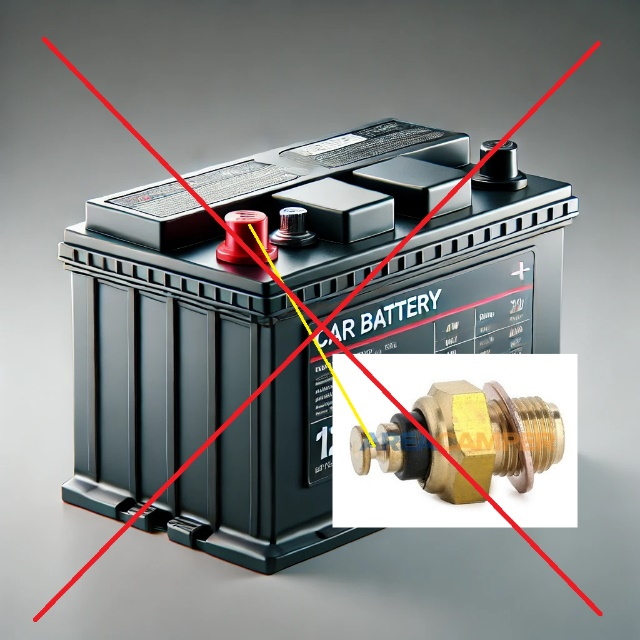
\includegraphics[width=\linewidth]{digifiz_manual/image002.jpg}
        \caption{Warning about applying external voltage to sensor circuits.}
    \end{subfigure}
    \caption{Typical warning labels supplied with the wiring harness.}
\end{figure}

Treat the dashboards as precision electronics: avoid ESD, moisture, and mechanical shock, and never use sensor readings for automated vehicle control.

\chapter{Operating Principle} \label{ch:operating-principle}

Digifiz Replica dashboards reuse the original Volkswagen enclosure, the factory CE~1 or CE~2 connectors, and either the mechanical speedometer cable or an electronic speed sensor.
Replica main boards are based on a fiberglass PCB populated with discrete components controlled by an ATmega~2560 microcontroller and MAX~7219 indicator drivers.

Digifiz Replica Next builds on an ESP32-S3 system-on-chip and introduces a newly manufactured SLA-printed enclosure, a redesigned front panel and cover, and a connector adapter board.
The Next-generation display is illuminated by WS2812 addressable LEDs mounted behind the front frame, and the accompanying harness includes the electronic speed sensor by default.

Both generations share the same display layout and MFA pages, ensuring that installation procedures and day-to-day operation remain familiar between hardware revisions.


\mainmatter
\chapter{Design Principles} \label{ch:Design}

It is not like I stated the \emph{Principles} at the beginning and then tried to follow them.
They emerged more naturally.
So the causal structure is more like
\[
    \raisebox{-0.15ex}{\parbox[c]{6em}{\centering made some design choices}}
    \mspace{12mu} \text{and} \mspace{10mu}
    \parbox[c]{7em}{\centering implemented certain features}
    \quad\longleadsto{}\quad
    \parbox[c]{10em}{\centering recognized \\\textcolor{gray}{at first subconscious} overarching principles}~.
\]
Anyway, here they are.
\begin{definition}[Design Principles] \label{def:Design Principles}
    The main design \emph{Principles} are:
    \begin{itemize}
        \item \textbf{Elegance} --- Aim for a classy, typographically elegant layout.
        \item \textbf{Structure} --- Create a smart, easy-to-reference, and skimmable structure.
        \item \textbf{Clarity} --- Eliminate distractions and strive for clear explanations. \qedhere
    \end{itemize}
\end{definition}
\begin{remark}[Common Goal, Alternative Definition via Antiprinciples]
    There is also an alternative point of view.
    The common goal of \Nref*{def:Design Principles} is to minimize the following \emph{Antiprinciples}:
    \begin{itemize}
        \item We should be concise, and that means fewer pages, the better.
              Long blocks of text without noticeable space between paragraphs are preferred (the reader should go on a walk to have some breathing spacetime).
        \item Avoid creating distinct anchor points for important concepts, since an attentive reader should be able to extract them from blocks of text.
        \item Do not waste time referencing earlier discussions and reflecting on them from the current context and point of view, as the reader is anyway making such connections all the time. \qedhere
    \end{itemize}
\end{remark}

Each of these principles is somehow reflected in the design choices and features included (or omitted) in \TeXtured{}, see \Cref{ch:Features} for more details.

\begin{remark}[Disclaimer]
    The following is at places highly opinionated, and not applicable to all scenarios and use-cases.
    I tried to describe my reasons for specific design choices, with which you can certainly disagree.
    I hope that at least it can provoke more people \emph{(especially you!)} to contemplate about document creation, ideally resulting in production of documents with overall better quality.
\end{remark}

\chapter{Technical Characteristics} \label{ch:technical-characteristics}

Both dashboard generations operate from the vehicle's 9--16~V electrical system.
Replica Next draws approximately 13~mA from the battery while powered down, whereas the classic Replica consumes no standby current when fully switched off.

\section{Measurement Capabilities}

\begin{itemize}
    \item \textbf{Vehicle speed:} measured through the mechanical or electronic speed sensor.
          The absolute error is 10~km/h, the relative error 3~km/h, and the indication saturates at 999~km/h (or mph for imperial units).
    \item \textbf{Engine speed:} derived from the ignition signal via an RC-limited optocoupler stage (430~nF/1.2~k\ohm{} with diode clamping).
          The absolute and relative errors are within 200~rpm.
    \item \textbf{Fuel level:} read from the resistive tank sender with an uncertainty of approximately 10~litres.
    \item \textbf{Coolant temperature:} displayed qualitatively using the OEM thermistor connected through the vehicle harness.
    \item \textbf{Time:} maintained to within one minute.
          Replica employs a DS3231 real-time-clock module with a CR2032 backup cell; Replica Next keeps time through firmware.
    \item \textbf{Indicator lamps:} direction indicators, high beam, oil pressure warnings, generator status, handbrake, rear window heating or diesel glow-plug, and front/rear fog lights.
\end{itemize}

\chapter{Operating Conditions and Safety Precautions} \label{ch:operating-conditions}

\section{Environmental Limits}

\begin{itemize}
    \item Ambient operating range: \(-40\,^{\circ}\mathrm{C}\) to \(+70\,^{\circ}\mathrm{C}\) with up to 95\% relative humidity.
    \item Year-round use inside the passenger compartment is supported, including long-term parking.
    \item Store the dashboard inside the vehicle cabin or in a dry indoor space between \(+15\,^{\circ}\mathrm{C}\) and \(+40\,^{\circ}\mathrm{C}\), protected from direct sunlight.
\end{itemize}

\section{Responsibilities and Limitations}

\begin{itemize}
    \item Digifiz dashboards are enthusiast devices intended for project cars; they are not certified measuring instruments.
    \item Installations are performed at the owner's risk.
          When readings appear questionable, verify them with factory gauges or independent instruments.
    \item Do not feed Digifiz measurements into automated vehicle control systems.
    \item The authors guarantee the documented functionality during a one-year warranty period for installations performed jointly and for two weeks on self-installations; malfunctions within these windows will be repaired.
\end{itemize}

\chapter{Preparation for Work and Work Order} \label{ch:preparation}

\section{Preparing the Vehicle}

Follow the sequence below when replacing the factory cluster:
\begin{enumerate}
    \item Remove the plastic trim covering the pedals and dashboard to expose the instrument cluster.
    \item Disconnect the vehicle battery.
    \item Unplug the factory harness from the instrument panel.
    \item Disconnect the mechanical speedometer cable (if fitted).
    \item Unscrew the cluster from its brackets and carefully remove it from the vehicle.
    \item Route the temperature and speed sensor harnesses supplied with the Digifiz kit.
    \item Install the new dashboard into the bracket grooves and secure it with screws.
    \item For Replica Next, connect the Volkswagen MFA sensors or compatible replacements and route the cables to the CE~1/CE~2 connectors.
    \item On single-connector variants (\texttt{GACS}/\texttt{GARS}/\texttt{DARS}/\texttt{DACS}), manually connect the labelled MFA\_MODE, MFA\_RESET, MFA\_BLOCK, and handbrake wires if the vehicle harness lacks these contacts.
    \item Plug in the harness(es) and connect the electronic speed sensor or speedometer cable as required.
    \item Reinstall the dashboard trim and pedal cover in the reverse order.
\end{enumerate}

\section{Working with the Instrument Panel}

The dashboard powers up automatically with ignition.
During the self-test the speed scale illuminates fully before stabilising at the current RPM value; the sidelights control the backlight.
Once the vehicle begins moving, the MFA controller updates the measurements described in \Cref{ch:technical-characteristics}.

\section{MFA Functions}

Six MFA pages are available:
\begin{enumerate}
    \item Daily operating time.
    \item Trip distance.
    \item Fuel consumption (not implemented on the first Replica revision).
    \item Average speed (displayed as the value multiplied by ten).
    \item Engine oil temperature (external harness required).
    \item Ambient temperature (external harness required).
\end{enumerate}

On classic Replica dashboards a capacitive touch point behind the VW badge cycles the pages.
Replica Next relies on an external steering column switch.
Touch durations behave as follows:
\begin{itemize}
    \item Short press (\(<1\)~s): cycle to the next MFA function.
    \item Medium press (1--3~s, when no steering column switch is present): switch between MFA memory blocks.
    \item Long press (3--7~s): reset the active MFA function (affecting consumption, trip distance, elapsed time, and average speed).
\end{itemize}

\section{Backlight Control and Indicator Layout}

Classic dashboards provide a manual brightness trim above the parking-light switch, whereas Replica Next relies on automatic brightness using an onboard photodiode.
Automatic control can be overridden through configuration commands described in \Cref{ch:replica-next-setup}.

The layout of the horizontal indicator block and the on-screen labelling are shown in \Cref{fig:indicator-layout,fig:indicator-legend}.

\begin{figure}[htbp]
    \centering
    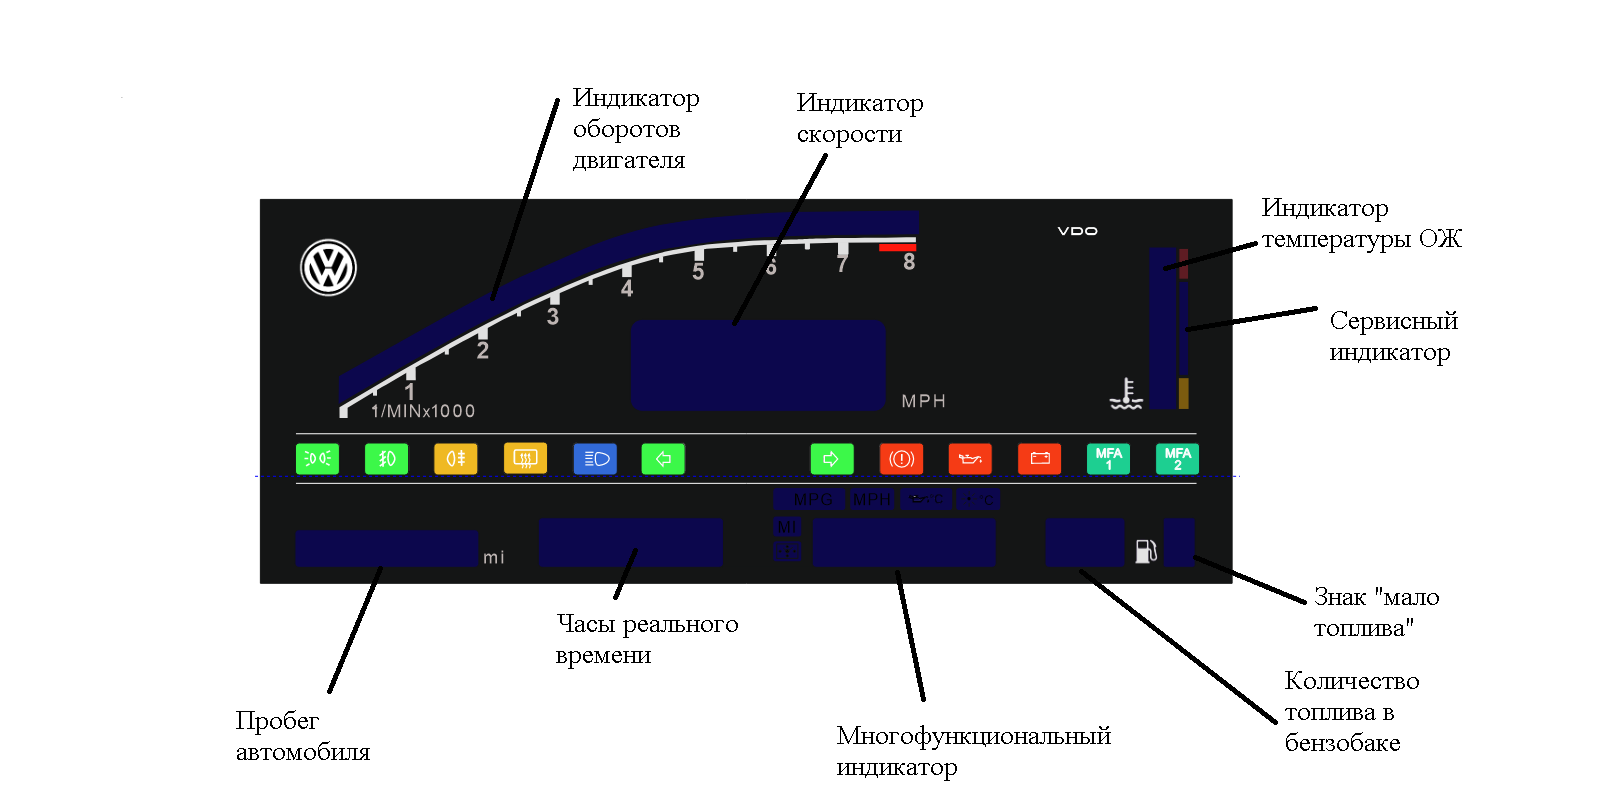
\includegraphics[width=0.85\textwidth]{digifiz_manual/image017.png}
    \caption{Indicator layout displayed during the power-on self-test.}
    \label{fig:indicator-layout}
\end{figure}

\begin{figure}[htbp]
    \centering
    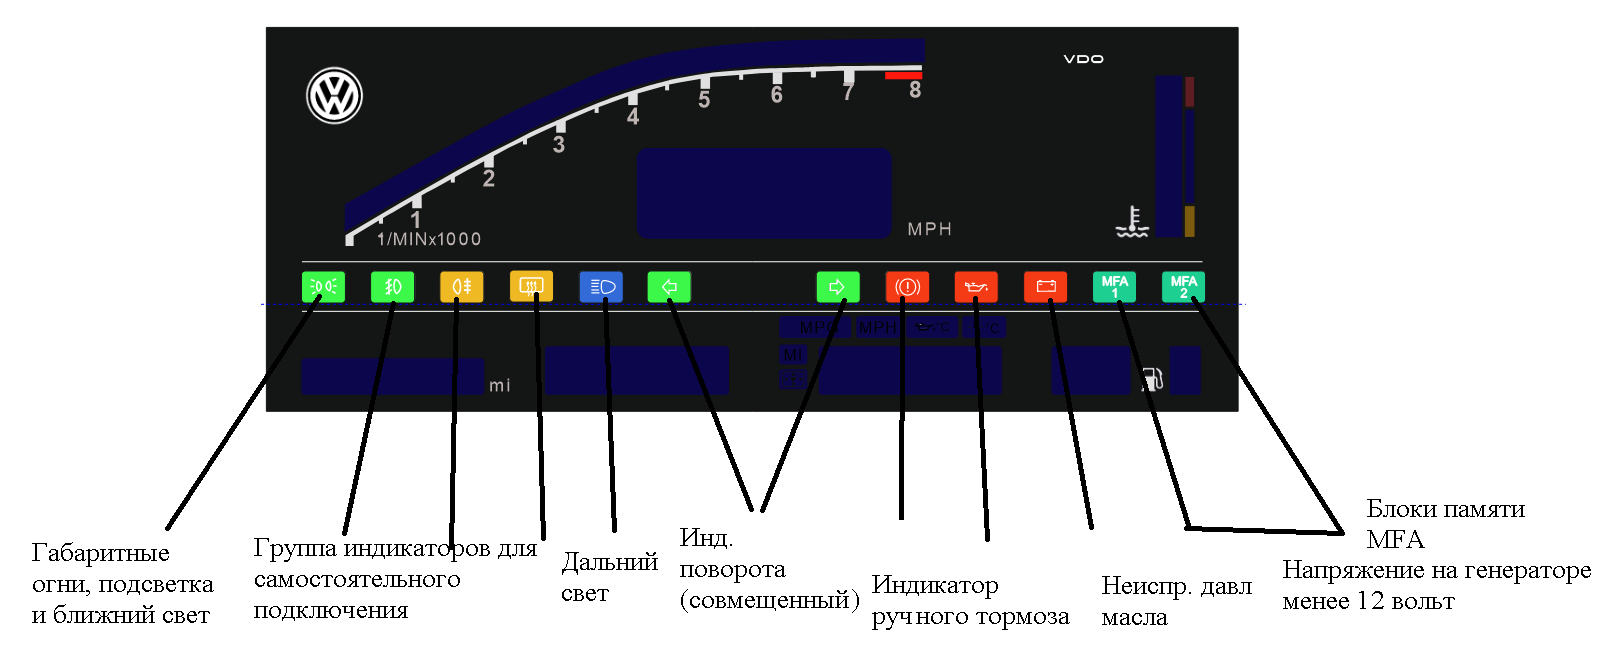
\includegraphics[width=0.8\textwidth]{digifiz_manual/image018.png}
    \caption{Legend for the horizontal indicator group.}
    \label{fig:indicator-legend}
\end{figure}

\section{Configuration Interfaces}

Both generations provide maintenance interfaces:
\begin{itemize}
    \item Classic Digifiz Replica units include a Bluetooth 2.0 (or BLE-compatible) module.
          Install the \emph{Serial Bluetooth Terminal} application from Google Play, pair with the dashboard, and issue commands directly from the terminal view.
          Apple iOS devices cannot connect to the module.
    \item Replica Next exposes an embedded Wi-Fi access point that serves the configuration portal detailed in \Cref{ch:replica-next-setup}.
          Disable mobile data while connecting to ensure the captive portal loads correctly.
\end{itemize}

Both generations also accept configuration commands over the USBasp programming interface when the dashboard is connected to a computer, which powers the unit for bench testing.

\chapter{Features of \TeXtured{}} \label{ch:Features}

In the following sections, we will describe the features of \TeXtured{} template, implemented by utilizing various \LaTeX{} packages and custom macros.

\begin{remark}[Packages and Macros]
    We will refer to various \LaTeX{} packages and macros using the following styles:
    \begin{itemize}
        \item \package{package} --- a package (together with a link to its \textsf{CTAN} page),
        \item \macro{\macro} --- a command/macro, either built-in or provided by a package,
        \item \custommacro{\custommacro} --- a custom macro defined in the \TeXtured{} template. \qedhere*
    \end{itemize}
\end{remark}

\section{Code Organization}%
\label{sec:Code Organization}

To avoid large and hard to navigate preamble files, the code is organized into multiple directories/files in the \path{preamble/} directory, each focusing on a particular function/feature, see \Cref{fig:preamble-file-structure}.
\begin{figure}[!ht]
    \fcapside[\FBwidth]{%
        \captionsetup{parskip = .5\baselineskip plus 1pt}%
        \caption[Structure of Preamble Directory]{%
            Structure of the \path{preamble/} directory.

            It is critical that the \path{preamble/pdfA-compliance/glyphtounicode.tex} file ensuring the PDF/A compliance is sourced before \fakemacro{\documentclass}.

            The \path{preamble/toggles.tex} files defines various toggles, which should be appropriately set right after.
            Finally, the rest of \grayenclose{preamble} files are then loaded through the \path{preamble/main.tex} file.

            When possible, add your own tweaks and macros to the \path{preamble/user/} directory reserved for this purpose.
            This way, you can easily update to newer versions of \TeXtured{} (hopefully) without conflicts.
        }%
        \label{fig:preamble-file-structure}%
    }{%
        \begin{tikzpicture}[dirtree]
            \node[directory] {preamble/}
            child { node {bibliography.bib}}
            child { node {data.tex}}
            child { node {toggles.tex}}
            child { node {main.tex}}
            child { node[directory] {debug/...}
                % child { node {commands.tex}}
                % child { node {line-numbers.tex}}
            }
            % child [missing] {} child [missing] {}
            child { node[directory] {environments/...}
                % child { node {init.tex}}
                % child { node {remark-like.tex}}
                % child { node {theorem-like.tex}}
                % child { node {todo-like.tex}}
            }
            % child [missing] {} child [missing] {} child [missing] {} child [missing] {}
            child { node[directory] {general/...}
                % child { node {colors.tex}}
                % child { node {floats.tex}}
                % child { node {hyperref.tex}}
                % child { node {typesetting.tex}}
            }
            % child [missing] {} child [missing] {} child [missing] {} child [missing] {}
            child { node[directory] {hacks/...}
                % child { node {custom-reference-boxes.tex}}
                % child { node {fix-qed.tex}}
                % child { node {floatrow-parskip.tex}}
            }
            % child [missing] {} child [missing] {}
            child { node[directory] {layout/...}
                % child { node {geometry.tex}}
                % child { node {headers.tex}}
                % child { node {numbering.tex}}
                % child { node {titles.tex}}
                % child { node {toc.tex}}
            }
            % child [missing] {} child [missing] {} child [missing] {} child [missing] {} child [missing] {}
            child { node[directory] {math/...}
                % child { node {fonts.tex}}
                % child { node {macros.tex}}
                % child { node {packages.tex}}
                % child { node {spacing.tex}}
            }
            % child [missing] {} child [missing] {} child [missing] {} child [missing] {}
            child { node[directory] {misc/...}
                % child { node {inkscape.tex}}
                % child { node {macros.tex}}
                % child { node {tikz.tex}}
            }
            % child [missing] {} child [missing] {} child [missing] {}
            child { node[directory] {pdfA-compliance/...}
                % child { node {glyphtounicode.tex}}
                % child { node[directory] {LaTeX-find-glyph-name/}
                %     child { node {LaTeX-find-glyph-name.tex}}
                % }
            }
            % child [missing] {} child [missing] {} child [missing] {}
            child { node[directory] {references/...}
                % child { node {backref.tex}}
                % child { node {biblatex-extra-fields.dbx}}
                % child { node {biblatex.tex}}
                % child { node {cite.tex}}
                % child { node {doi-eprint-url.tex}}
                % child { node {fields.tex}}
                % child { node {style.tex}}
            }
            % child [missing] {} child [missing] {} child [missing] {} child [missing] {} child [missing] {} child [missing] {} child [missing] {}
            child { node[directory] {user/...}
                % child { node {macros.tex}}
                % child { node {math.tex}}
            }
            % child [missing] {} child [missing] {}
            ;
        \end{tikzpicture}%
    }
\end{figure}

\begin{remark}[Pointers to Directories/Files]
    If you want to tweak some aspect of the template --- or learn how a given feature is implemented --- pointers to the relevant directories/files are provided next to the subsequent section/subsection titles to help you navigate the code.
\end{remark}

\begin{remark}[Custom User Macros]
    Store your own macros in the \path{preamble/user/} directory, which is reserved precisely for this purpose.
    Then, if you would like to update to a newer version of \TeXtured{}, you will be having easier time --- less mixing of your code with the template code will result in fewer conflicts you must resolve manually.
\end{remark}

\begin{remark}[Auxiliary Files]
    To avoid cluttering the directories with \emph{auxiliary files} generated during the compilation, it is recommended to use the \macro{aux_dir} setting in the \path{.latexmkrc} file (enabled by default, the \macro{aux_dir} being \path{.aux/}).
    All auxiliary files are then stored in a separate directory, leaving the rest tidy.
\end{remark}

\begin{remark}[Suggestion: One Sentence Per Line]
    It is a good practice to follow \enquote{one sentence per line} rule (or something similar), since it improves diffs for versioning systems like \texttt{git}.
    Tools like \texttt{latexindent} can help.
    \begin{Note}
        My config for \texttt{latexindent} mostly works, but some corner cases can surface.
        Will share someday.
    \end{Note}
    If multiple sentences are on the same line, changing just one word results in the whole line being marked as changed, making it harder to see how much the text was actually changed in a given commit.
\end{remark}



\section{Page Layout and Style}%
\label{sec:Page Layout}
\dirTeXtured{preamble/layout/}

We will first describe the page layout and style, which includes page dimensions, headers and footers, page numbering, and heading style.

\subsection{Page Dimensions, Printing Layout}%
\label{sub:Page Dimensions}
\fileTeXtured{preamble/layout/geometry.tex}

Using \package{geometry} package --- set up the page layout (supported single/double-sided printing).
Apply \macro{\flushbottom} --- try to make text body on all pages have the same height.

\subsection{Page Headers and Footers}%
\label{sub:Headers Footers}
\fileTeXtured{preamble/layout/headers.tex}

Using \package{fancyhdr} package --- page headers and footers --- consistent style also for initial page of a chapter (not totally different style with numbering in the bottom center \ldots).

\subsection{Page Numbering}%
\label{sub:Page Numbering}
\fileTeXtured{preamble/layout/numbering.tex}

Placing custom \custommacro{\frontmatter}, \custommacro{\mainmatter}, and \custommacro{\backmatter} macros at appropriate places in \path{thesis.tex}, \emph{Roman numbering} is set up for \emph{front matter}, that is until the start of first numbered chapter, and then \emph{Arabic numbering} for the rest of the document.


\subsection{Heading Style}%
\label{sub:Heading Style}
\fileTeXtured{preamble/layout/titles.tex}

Pretty chapter heading style --- big calligraphic number/letter behind the title.


\section{Sane Typographical Defaults}%
\label{sec:Sane Typographical Defaults}
\dirTeXtured{preamble/general/}

Now we will concern ourselves with more intricate and detailed typography, more at level of paragraphs, sentences, words, and even letters.

\subsection{Paragraphs}%
\label{sub:Paragraphs}
\fileTeXtured{preamble/general/typesetting.tex}

No paragraph indentation, proper space between paragraphs --- \package{parskip}.

\subsection{Floats, Captions}%
\label{sub:Floats_Captions}
\fileTeXtured{preamble/general/floats.tex}

Caption styling includes a slight hang, \macro{\footnotesize} font, and a bold sans label.
See \Cref{appendix:example} for a showcase of the different caption types.


\subsection{Font and Related Stuff}%
\label{sub:Font}
\fileTeXtured{preamble/general/typesetting.tex}

The default choice are \emph{Latin Modern} fonts --- a classic really.
Various families and shapes are typically used for different purposes:
\begin{itemize}
    \item \emph{Serif} family for the main text
    \item \emph{Slanted} shape for emphasis using \macro{\emph} macro (instead of the default \emph{Italic} shape, which is reserved mainly for math formulas)
          \begin{remark}[Nested Emphasis]
              Nested emphasis is displayed in \emph{Italic} shape.
              It is rather rare to nest an \emph{additional \emph{emphasis} inside an emphasis}.
          \end{remark}
    \item \emph{(Bold) Sans} family for headings and other structural elements
    \item \emph{Typewriter} family for computer code and similar stuff
\end{itemize}
\vspace{1ex}

\begin{example}
    Quick showcase of some font families and shapes:\par \leftskip=1em

    {                  This is Latin Modern Serif \(\alpha = 2^{2}\)}\\
    {\slshape          This is Latin Modern Serif Oblique \(\alpha = 2^{2}\)}\\
    {\bfseries         This is Latin Modern Serif Bold \(\alpha = 2^{\bm{{2}}}\)}\\
    {\bfseries\slshape This is Latin Modern Serif Bold Oblique \(\alpha = 2^{2}\)}

    {\sffamily                  This is Latin Modern Sans \(\alpha = 2^{2}\)}\\
    {\sffamily\slshape          This is Latin Modern Sans Oblique \(\alpha = 2^{2}\)}\\
    {\sffamily\bfseries         This is Latin Modern Sans Bold \(\alpha = 2^{2}\)}\\
    {\sffamily\bfseries\slshape This is Latin Modern Sans Bold Oblique \(\alpha = 2^{2}\)}
\end{example}
\begin{Note}
    Sans math font has problems with showing properly all bold symbols (sub/superscripts don't work automatically).
\end{Note}

For consistent quotation use \macro{\enquote} macro provided by \package{csquotes}.

\subsection{\texorpdfstring{Micro-\!Typography}{Micro-Typography}}%
\label{sub:Micro-Typography}
\fileTeXtured{preamble/general/typesetting.tex}

Enable micro-typographic extensions with package \package{microtype}, most prominently character protrusion and font expansion.

Following quote from \package{microtype} documentation nicely explains what it is about:
\begin{displayquote}
    Micro-typography is the art of enhancing the appearance and readability of a
    document while exhibiting a minimum degree of visual obtrusion.
    It is concerned with what happens between or at the margins of characters, words or lines.
    Whereas the macro-typographical aspects of a document (i.e., its layout) are clearly visible even to the untrained eye, micro-typographical refinements should ideally not even be recognizable.
    That is, you may think that a document looks beautiful, but you might not be able to tell exactly why: good micro-typographic practice tries to reduce all potential irritations that might disturb a reader.
\end{displayquote}


\section{Document Structure}%
\label{sec:Document Structure}

It is important to have a clear and consistent structure of the document.
This can be achieved by using various environments for different types of content, and by providing clear and informative titles for each part of the document, thus making it easier to navigate and understand.

\subsection{Structure Environments}%
\label{sub:Structure Environments}
\fileTeXtured{preamble/environments/*.tex}
% \fileTeXtured{preamble/environments/init.tex}
% \fileTeXtured{preamble/environments/theorem-like.tex}
% \fileTeXtured{preamble/environments/remark-like.tex}
% \fileTeXtured{preamble/environments/todo-like.tex}

Inspired by the structured mathematical texts, enclosing various parts of the document in the corresponding environments can help to make the document more structured and easier to read.
Implemented mostly \package{tcolorbox} package and \package{keytheorems} (modern key--value interface for \package{amsthm}).

\begin{remark}[Default Environments]
    There are predefined boxed \enquote{theorem-like} environments for \textsf{Definition}, \textsf{Theorem}, \textsf{Lemma}, \textsf{Corollary}, \textsf{Proposition},
    and non-boxed \enquote{remark-like} environments for \textsf{Remark}, \textsf{Proof}, \textsf{Example}, \textsf{Derivation}, \textsf{Calculation}, \textsf{Idea}, and \textsf{Tip} (these have at least a mark indicating the end of the environment).

    Names of the corresponding environments are lowercase, for example \texttt{definition}, \texttt{remark}, and so on.
    They also accept an optional argument for a short description.
\end{remark}

Some additional points about the \emph{structure environments}:
\begin{itemize}
    \item provide clear structure, enables high level of interlinking
    \item they make the text easy to skim through, quickly get an idea, and know roughly what to expect
    \item have shared numbering, together with tables, figures, equations --- leads to a linear increase of the reference number, making them easier to locate
    \item not only for physics/math texts, can be generally used to highlight key ideas
          \begin{tip}[Custom Structure Environments]
              You can easily create additional \enquote{structure} environments, see \Cref{sec:Structure}.
          \end{tip}
    \item avoid using emphasis for the whole body of \enquote{theorem-like} environments, since we already have a whole box around it to make them stand out
\end{itemize}
\vspace{1ex}

\begin{remark}
    There are also helper environments for \textsf{Todo}-like notes.
    By default, there are \textsf{Todo}, \textsf{Note}, \textsf{Suggestion}, and \textsf{Question} environments, but you can easily create your own.

    To avoid conflicts with possible existing macros/environments, names of these environments are capitalized, for example \texttt{Todo}, \texttt{Note}, and so on.
\end{remark}

\begin{Note}
    No \enquote{code listing} setup yet.
    PRs welcome.
\end{Note}

\subsection{References and Links}%
\label{sub:References Links}
\fileTeXtured{preamble/hacks/custom-reference-boxes.tex}

Custom reference/link/citation styles using \package{tcolorbox} package.
\begin{Note}[Slight Inconvenience --- Line Breaks]
    There is a slight inconvenience due to small flexibility around line breaks.
    It would be nice to have a proper workaround.
\end{Note}
\begin{remark}[Rationale]
    I like to have clearly distinguished references, links, and citations.
    By default, \package{hyperref} provides frames around links, but they are not that pretty, and the PDF viewer must support them.
    Using just colors can sometimes look better, but I still wasn't satisfied.

    Sometimes it is nice to know the precise location of the reference, especially when the document is printed and you cannot simply click on them.
    Therefore, the page number is (by default) included with \custommacro{\Cref}, see \Cref{rem:zref-clever}.
    Use the starred variant \custommacro{\Cref*} to omit it.
\end{remark}
\begin{remark}[Automatic Reference Type Detection] \label{rem:zref-clever}
    Package \package{zref-clever} provides \macro{\zcref} command --- similarly to the older, no longer maintained, \package{cleveref} package --- which automatically detects the type of reference, and formats it accordingly.
    This behavior is adapted in \TeXtured{} with the macro \custommacro{\Cref}, which wraps the link in nice box, and also shows a corresponding page number of the target.

    If you want the link to show the reference title, use \custommacro{\Nref} --- or the starred variant \custommacro{\Nref*} to omit the page number --- which utilizes \package{zref-titleref}.
\end{remark}

\subsection{Table of Contents and Outline/Index}%
\label{sub:Table of Contents and Index}
\fileTeXtured{preamble/layout/toc.tex}

Clear and elegant Table of Contents, which includes all the important parts --- also \grayenclose{unnumbered} subsections, but in a more compact style.

Similarly, automatically populate the PDF Outline/Index (digital Table of Contents in PDF viewer).
It is very handy for navigating longer documents, and includes also other important pages other than just initial pages of main chapters: Title Page, Contents, Introduction, References, and so on.
\begin{remark}
    I use \texttt{Zathura} as my PDF viewer, with the Outline/Index just one \macro{Tab} away, allowing me to quickly jump to the desired part of the document.
\end{remark}

\begin{remark}[List of Figures, Tables, \ldots{}]
    If you want/need to include a List of Figures, List of Tables, and so on, you can easily do so by uncommenting the relevant lines in the \custommacro{\contentsandlists} macro.
\end{remark}


\section{Bibliography/References}%
\label{sec:Bibliography/References}
\dirTeXtured{preamble/references/}

Pretty and functional Bibliography/References, via \package{biblatex} package.

\subsection{Bibliography Style}%
\label{sub:Bibliography Style}
\fileTeXtured{preamble/references/*.tex}
% \fileTeXtured{preamble/references/biblatex.tex}
% \fileTeXtured{preamble/references/style.tex}
% \fileTeXtured{preamble/references/fields.tex}

Entries in \Nref{ch:References} have a clean consistent style, which builds on the \macro{ext-numeric-verb} style from \package{biblatex-ext} package.

\begin{tip}[Bibliography Data]
    Make sure to gather all the relevant data you need for every reference.
    If you later decide you want to reduce the amount of presented information, \package{biblatex} can help you with that.
    For example, it is possible to automatically
    \begin{itemize}
        \item remove \macro{url} field if \macro{doi} field is present,
        \item ignore unwanted fields (\macro{pages}, \macro{number}, \macro{volume}, \macro{series}, \macro{location}, \ldots). \qedhere*
    \end{itemize}
\end{tip}

\subsection{Extra Fields}%
\label{sub:Extra Fields}
\fileTeXtured{preamble/references/biblatex-extra-fields.dbx}

Support extra \custommacro{github} field.

\subsection{Custom External Links}%
\label{sub:Custom External Links}
\fileTeXtured{preamble/references/doi-eprint-url.tex}

Have the external \textsf{DOI/arXiv/URL/GitHub} links displayed in custom boxes, and place them on the new line.

\subsection{Backreferences}%
\label{sub:Backreferences}
\fileTeXtured{preamble/references/backref.tex}

Include \emph{backreferences}, which point from the bibliography to the pages where the reference was cited.

\subsection{Citation Style}%
\label{sub:Citation Style}
\fileTeXtured{preamble/references/cite.tex}

Include \texttt{[} and \texttt{]} characters around citation number inside the link (and wrap in \package{tcolorbox} \ldots), for example \autocite{TeXtured}.


\section{PDF/A Compliance}%
\label{sec:PDF/A Compliance}
\dirTeXtured{preamble/pdfA-compliance/}

Proper metadata setup (via \package{hyperref} and \macro{\DocumentMetadata}).
\begin{remark}[Document Data]
    Various data about the work should be entered in \path{preamble/data.tex} file.
    When the relevant entries contain \LaTeX{} commands (for example to obtain specific formatting of the title), it is necessary to provide \enquote{plaintext} variations, so that \package{hyperref} can properly set up PDF metadata.
\end{remark}

Next we will describe various common violations of PDF/A standard, and how to fix them.

\subsection{Glyph to Unicode Map}%
\label{sub:Glyph to Unicode Map}
\fileTeXtured{.../pdfA-compliance/glyphtounicode.tex}
% \fileTeXtured[0ex]{preamble/pdfA-compliance/glyphtounicode.tex}

To obtain PDF/A compliant PDF, we need to have Unicode mapping for all glyphs used in the document.
It can happen --- mainly when using fonts providing extra mathematical symbols --- that certain glyphs are not covered by mappings loaded in \path{preamble/pdfA-compliance/glyphtounicode.tex}.

In the \path{preamble/pdfA-compliance/glyphtounicode.tex} file you can also find an example \textsf{veraPDF} output for a PDF with a problematic glyph.
It also points to a guide located in \path{preamble/pdfA-compliance/LaTeX-find-glyph-name/} directory, which explains how to find out the glyph name, and how to provide the \emph{glyph to Unicode} mapping with \macro{\pdfglyphtounicode} command.


\subsection{PDF \texorpdfstring{\fakemacro{/Interpolation}}{/Interpolation} Key}%
\label{sub:PDF Interpolation Key}

Some PDFs can have enabled the \macro{/Interpolation} key, for example \texttt{Inkscape} generated PDFs with blur parts.
However, PDF/A requires it to be disabled.

This is automatically fixed by \path{figures/Inkscape/inkscape-export-to-latex} shell script.


\section{Miscellaneous}%
\label{sec:Miscellaneous}

\subsection{Math-Related Tweaks --- \texorpdfstring{\rmfamily\(\E^{\I\pi}\)}{exp(iπ)}}%
\label{sub:Math Macros}
\fileTeXtured{preamble/math/}

Some of the math-related tweaks:
\begin{itemize}
    \item Use \macro{\boldmath} automatically for \macro{\textbf} text (useful mainly in headings).
    \item Possible to use sans italic font for math via \custommacro{\mathsfit}.
    \item Better extendable arrows with \package{TikZ}.
    \item \emph{(Optional, disabled by default)} Automatically change usage of \macro{\textcolor} to \macro{\mathcolor} in math mode, so that we get proper math spacing, for example
          \[ a \mathcolor{gray}{\times} b \text{ (right spacing)} \qquad\text{versus}\qquad a \textcolor{gray}{\times} b \text{ (wrong spacing)}\eqend \]
          However, it is recommended to explicitly use \macro{\mathcolor} when appropriate, since it leads to easier maintenance of the code (copy-pasting to other projects will work without problems).
\end{itemize}

\vspace{1ex}
Following practice is highly recommended.
\begin{tip}[Define Your Own Math Macros]
    Frequently define macros for notation used more than once. Advantages are for example:
    \begin{itemize}
        \item Code is easier to read/write, since it is more \enquote{semantic}.
        \item To tweak notation, you only need to change it in one place.
        \item Easier to find all occurrences of a certain notion. \qedhere
    \end{itemize}
\end{tip}

\subsection{GitHub Actions}%
\label{sub:GitHub Actions}
\fileTeXtured{.github/workflows/}

Describe implemented \textsf{GitHub Actions}:
\begin{itemize}
    \item Automatic \texttt{latexmk} build of the latest PDF version.
    \item PDF/A verification via \textsf{veraPDF}.
    \item Deploy to \texttt{gh-pages} branch.
          One can furthermore enable (in repo settings) \textsf{GitHub Pages} for \texttt{gh-pages} branch, which will automatically upload latest PDF to \texttt{https://username.github.io/reponame/thesis.pdf}.
          This enables convenient sharing of your (even continuously evolving) work without needing to commit the PDF (resulting in large repository size) or compiling the PDF on the receiving side.
          \begin{remark}[Private Repositories]
              Even for private repositories such link is publicly accessible.
              This is why \textsf{GitHub Pages} setup is not done automatically for you.
              If you want to share the work more \enquote{privately}, there are other solutions, for example \textsf{GitHub Action} which uploads PDF to \textsf{Google Drive}, and sharing via a private link.
              Also look at \Cref{sub:Censoring}.
          \end{remark}
\end{itemize}

\subsection{Censoring}%
\label{sub:Censoring}
\fileTeXtured{preamble/debug/censor.tex}

Censoring/redaction using \package{censor} package.
Use \macro{\censor} or \macro{\censorbox}.
For example, censor the following sentence: \censor{\TeXtured{} is an amazing template!}.

\subsection{\texorpdfstring{\texttt{Inkscape}}{Inkscape} Integration}%
\label{sub:Inkscape Integration}
\fileTeXtured{preamble/misc/inkscape.tex}

\begin{itemize}
    \item automatic export after changing the \texttt{svg} (need to enable \macro{--shell-escape} for \hologo{pdfTeX} or \hologo{LuaTeX}, done via \path{.latexmkrc})
    \item watermark via \texttt{ps} injection
          \begin{remark}[Watermark String]
              Edit the watermark text in the shell script \path{figures/Inkscape/inkscape-export-to-latex} to your liking.
          \end{remark}
          \begin{Todo}
              Make it easier to change the watermark text.
              Or extract it somehow automatically from the PDF document?
          \end{Todo}
    \item automatic fix of \macro{/Interpolation} key problem
\end{itemize}


\section{Non-Features}%
\label{sec:Non-Features}

These features were deemed unnecessary, or even counterproductive, and thus were not implemented/not customized.
This does not mean that it is hard or not compatible to use them with \TeXtured{}.

\subsection{Footnotes}%
\label{sub:Footnotes}

\begin{itemize}
    \item they break the flow of reading, can be distracting
    \item either it is important and you want it there --- no need to use footnotes --- or it is not so important (maybe just a reminder/remark), but then there are in my opinion better ways to handle such situation
          \begin{itemize}
              \item grayed out/smaller text, sidenotes are better alternative, if the page layout enables them
              \item it is not bad to remind reader of something in the main text\ldots
          \end{itemize}
\end{itemize}

\subsection{Index, Glossary}%
\label{sub:Index Glossary}

\begin{itemize}
    \item since the text is primarily intended for electronic use, finding usage of certain terms is easy
    \item text should be ideally structured in such a way, that finding definitions of important terms is straightforward --- interlinking/referencing in proper places to indicate where the notion to be used was defined/discussed
\end{itemize}

\chapter{Troubleshooting and Adjustments} \label{ch:Tips}

This chapter summarises common configuration and troubleshooting scenarios reported for Digifiz Replica Next and classic Digifiz Replica dashboards.
Each entry lists the recommended diagnostic steps and the configuration commands involved.

\section{Replica Next}

\begin{description}
    \item[Hotspot not visible] Move closer to the dashboard and ensure the vehicle is in an open area. Disable cellular data and reconnect to \texttt{Digifiz\_AP} (or \texttt{PHOL-LABS2}).
    \item[404 when opening \texttt{192.168.4.1}] Confirm that mobile data is disabled and retry the connection.
    \item[Firmware updates] Navigate to the \emph{WiFi} tab, select the provided \texttt{Digifiz.bin} release (latest builds are published at \url{https://github.com/Sgw32/DigifizReplica/releases}), click \emph{Upload}, and repeat if the upload fails. Record the current odometer value and restore it with command \verb|11 <mileage>| after the update if necessary.
    \item[Commands ignored] Refresh the web page, reopen the \emph{Control} tab, and send the command again.
    \item[Speed reading incorrect] Connect via Wi-Fi, drive at an indicated 100~km/h, note the GPS speed, then issue \verb|1 <gps_value>| (for example, \verb|1 85|) to adjust \texttt{PARAMETER\_SPEEDCOEFFICIENT}.
    \item[RPM reading incorrect] Issue \verb|22 <value>| (for example, \verb|22 1500| to halve the reading) to recalibrate \texttt{PARAMETER\_RPMCOEFFICIENT}. Audi clusters typically use \verb|22 3000|.
    \item[Display too dim] Disable automatic brightness with \verb|13 0| and increase manual brightness (for example, \verb|14 50|). Use conservative values (below 60) to extend LED life.
    \item[Setting the clock] From the web terminal (or Serial Bluetooth Terminal on legacy builds), enter \verb|255 <hours>| followed by \verb|254 <minutes>| (for example, \verb|255 23| and \verb|254 55|).
    \item[Fuel level stuck at zero or maximum] Disconnect the battery, verify that the sender resistance measured between the harness pin and vehicle ground is within 30--300~\ohm{}, and inspect the connector for continuity. Short circuits (<5~\ohm{}) must be eliminated. If the resistance varies correctly but the gauge does not, capture \verb|adc 0| readings at multiple fuel levels and share them with the authors.
    \item[Fuel flow readings inaccurate] The optional flow sensor delivers emulated data and is unreliable without the manifold pressure sensor; treat the readings as experimental.
    \item[Coolant temperature scaling] Adjust \texttt{PARAMETER\_COOLANT\_MIN\_R} and \texttt{PARAMETER\_COOLANT\_MAX\_R} to tune the display range (for example, \verb|27 30| lowers the ``1~bar'' threshold to 30~\,^{\circ}C).
    \item[Oil or ambient temperature missing] Disconnect the battery and measure the sensor resistance: oil sensors should read about 2~k\ohm{}, ambient sensors about 10~k\ohm{} at room temperature. If necessary, adjust \texttt{PARAMETER\_NORMAL\_RESISTANCE\_OIL} (command 20) or \texttt{PARAMETER\_NORMAL\_RESISTANCE\_AMB} (command 21); values below the default lower the indicated temperature, higher values raise it. Persistent issues should be escalated with \verb|adc 0| readings.
    \item[Changing UI colours] Use commands 31--33 to set the RGB components or update to the latest firmware to access the visual colour controls in the web UI.
\end{description}

\section{Classic Digifiz Replica}

\begin{description}
    \item[Bluetooth module not visible] Confirm that the host uses Bluetooth Classic rather than BLE. iOS devices cannot connect to the Bluetooth~2.0 module.
    \item[Commands rejected] Firmware builds from 2024 and newer require unlocking with \verb|234 123| before accepting configuration commands.
    \item[Speed or RPM calibration] Adjust \texttt{PARAMETER\_SPEEDCOEFFICIENT} with \verb|1 <gps_value>| and \texttt{PARAMETER\_RPMCOEFFICIENT} with \verb|0 <value>| or \verb|22 <value>|, using the same approach as Replica Next.
    \item[Manual brightness adjustment] Disable automatic brightness with \verb|13 0| and set \verb|14 15| for maximum brightness. Re-enable automatic control with \verb|13 1| if required.
    \item[Clock adjustment] Enter \verb|255 <hours>| followed by \verb|254 <minutes>| through Serial Bluetooth Terminal.
    \item[Fuel gauge issues] With the battery disconnected, verify the sender resistance on the harness (30--300~\ohm{}) and inspect for shorts. Check the signal path to the main board and clean contacts if needed.
    \item[Fuel flow accuracy] The optional flow sensor relies on intake manifold pressure data and otherwise produces approximate readings.
    \item[Coolant temperature calibration] Tune \texttt{PARAMETER\_COOLANT\_MIN\_R} and \texttt{PARAMETER\_COOLANT\_MAX\_R} experimentally to suit the vehicle (for example, \verb|27 30|).
\end{description}

For additional parameter defaults and configuration details, refer to \Cref{tbl:next-commands,tbl:next-defaults} and the classic Replica command list in \Cref{appendix:reference}.


\backmatter
%% NOTE: uncomment following line if you use parts in your document
% \addtocontents{toc}{\vspace{2ex}}  % Add extra space after the last part in TOC

\chapternotnumbered{Summary and Outlook}

Summary and Outlook.


\appendix
\chapter{Reference Tables} \label{appendix:reference}

\section{Classic \ReplicaGenOne{} Command Reference}

The classic Replica firmware shares most commands with \ReplicaNextShort{}.
Commands 31--33 (colour control) are only active on \ReplicaNextShort{} units; other commands apply equally to both generations.

\begin{table}[htbp]
    \centering
    \caption{Primary configuration commands for classic \ReplicaGenOne{} dashboards.}
    \label{tbl:replica-commands}
    {\scriptsize
    \begin{tblr}{
        colspec = {Q[c,0.16\linewidth] Q[l,0.5\linewidth] Q[l]},
        rowsep = 2pt,
    }
        \toprule
        \textbf{Command} & \textbf{Name} & \textbf{Description} \\
        \midrule
        22 (or 0) & \InlineCode{PARAMETER\_RPMCOEFFICIENT} & Engine RPM calibration factor. \\
        1  & \InlineCode{PARAMETER\_SPEEDCOEFFICIENT} & Speed calibration factor. \\
        2  & \InlineCode{PARAMETER\_COOLANTTHERMISTORB} & Coolant thermistor beta coefficient. \\
        3  & \InlineCode{PARAMETER\_OILTHERMISTORB} & Oil thermistor beta coefficient. \\
        4  & \InlineCode{PARAMETER\_AIRTHERMISTORB} & Ambient thermistor beta coefficient. \\
        5  & \InlineCode{PARAMETER\_TANKMINRESISTANCE} & Minimum fuel sender resistance. \\
        6  & \InlineCode{PARAMETER\_TANKMAXRESISTANCE} & Maximum fuel sender resistance. \\
        7--10 & \InlineCode{PARAMETER\_TAU\_\textit{X}} & Filtering constants for coolant, oil, air, and fuel level.
        \\
        11 & \InlineCode{PARAMETER\_MILEAGE} & Total odometer value. \\
        12 & \InlineCode{PARAMETER\_DAILY\_MILEAGE} & Trip odometer. \\
        13 & \InlineCode{PARAMETER\_AUTO\_BRIGHTNESS} & Automatic brightness enable. \\
        14 & \InlineCode{PARAMETER\_BRIGHTNESS\_LEVEL} & Manual brightness level. \\
        15 & \InlineCode{PARAMETER\_TANK\_CAPACITY} & Fuel tank capacity. \\
        16 & \InlineCode{PARAMETER\_MFA\_STATE} & Active MFA mode. \\
        17 & \InlineCode{PARAMETER\_BUZZER\_OFF} & Disable buzzer (Replica only). \\
        18 & \InlineCode{PARAMETER\_MAX\_RPM} & Tachometer scaling (7000 default). \\
        19--21 & \InlineCode{PARAMETER\_NORMAL\_RESISTANCE\_\textit{X}} & Sensor resistances at \SI{25}{\celsius} for coolant, oil, and ambient inputs. \\
        23 & \InlineCode{PARAMETER\_DOT\_OFF} & Clock colon behaviour. \\
        24 & \InlineCode{PARAMETER\_BACKLIGHT\_ON} & Enable backlight when low beam is active. \\
        25 & \InlineCode{PARAMETER\_M\_D\_FILTER} & Median filter constant. \\
        26 & \InlineCode{PARAMETER\_COOLANT\_MAX\_R} & Coolant sensor threshold for full-scale indication. \\
        27 & \InlineCode{PARAMETER\_COOLANT\_MIN\_R} & Coolant sensor threshold for ``1~bar'' indication. \\
        31--33 & \InlineCode{PARAMETER\_MAINCOLOR\_[RGB]} & UI colour components (\ReplicaNextShort{} only). \\
        37 & \InlineCode{PARAMETER\_RPM\_FILTER} & RPM filtering aggressiveness. \\
        128 & \InlineCode{PARAMETER\_READ\_ADDITION} & Add 128 to read the current value of a command. \\
        255 & \InlineCode{PARAMETER\_SET\_HOUR} & Set clock hours. \\
        254 & \InlineCode{PARAMETER\_SET\_MINUTE} & Set clock minutes. \\
        253 & \InlineCode{PARAMETER\_RESET\_DAILY\_MILEAGE} & Reset trip odometer. \\
        252 & \InlineCode{PARAMETER\_RESET\_DIGITAL} & Factory reset of stored parameters. \\
        \bottomrule
    \end{tblr}}
\end{table}

\section{Classic \ReplicaGenOneShort{} Default Values}

\begin{table}[htbp]
    \centering
    \caption{Default configuration for the classic \ReplicaGenOne{}.}
    \label{tbl:replica-defaults}
    {\scriptsize
    \begin{tblr}{
        colspec = {Q[l,0.55\linewidth] Q[c,0.16\linewidth] Q[l]},
        rowsep = 2pt,
    }
        \toprule
        \textbf{Parameter} & \textbf{Default} & \textbf{Notes} \\
        \midrule
        \InlineCode{PARAMETER\_RPMCOEFFICIENT} & 3000 &  \\
        \InlineCode{PARAMETER\_SPEEDCOEFFICIENT} & 100 &  \\
        \InlineCode{PARAMETER\_COOLANTTHERMISTORB} & 4000 &  \\
        \InlineCode{PARAMETER\_OILTHERMISTORB} & 4000 &  \\
        \InlineCode{PARAMETER\_AIRTHERMISTORB} & 3812 & 3600 on Gen~2. \\
        \InlineCode{PARAMETER\_TANKMINRESISTANCE} & 35 & Ohms. \\
        \InlineCode{PARAMETER\_TANKMAXRESISTANCE} & 265 & Ohms. \\
        \InlineCode{PARAMETER\_TAU\_COOLANT} & 2 &  \\
        \InlineCode{PARAMETER\_TAU\_OIL} & 2 &  \\
        \InlineCode{PARAMETER\_TAU\_AIR} & 2 &  \\
        \InlineCode{PARAMETER\_TAU\_TANK} & 2 &  \\
        \InlineCode{PARAMETER\_MILEAGE} & Vehicle-specific & Preserve existing odometer. \\
        \InlineCode{PARAMETER\_DAILY\_MILEAGE} & 0 &  \\
        \InlineCode{PARAMETER\_AUTO\_BRIGHTNESS} & 1 & Enabled. \\
        \InlineCode{PARAMETER\_BRIGHTNESS\_LEVEL} & 7 or 13 & Typical values for Gen~1/1.5. \\
        \InlineCode{PARAMETER\_TANK\_CAPACITY} & 63 & Litres. \\
        \InlineCode{PARAMETER\_MFA\_STATE} & 0 &  \\
        \InlineCode{PARAMETER\_BUZZER\_OFF} & 1 & Buzzer disabled. \\
        \InlineCode{PARAMETER\_MAX\_RPM} & 8000 & 7000 on earlier clusters. \\
        \InlineCode{PARAMETER\_NORMAL\_RESISTANCE\_COOLANT} & 1000 & \si{\ohm} at \SI{25}{\celsius}. \\
        \InlineCode{PARAMETER\_NORMAL\_RESISTANCE\_OIL} & 1000 & \si{\ohm} at \SI{25}{\celsius}. \\
        \InlineCode{PARAMETER\_NORMAL\_RESISTANCE\_AMB} & 2991 & \si{\ohm} at \SI{25}{\celsius}. \\
        \InlineCode{PARAMETER\_DOT\_OFF} & 0 & Blinking colon. \\
        \InlineCode{PARAMETER\_BACKLIGHT\_ON} & 1 & Enabled. \\
        \InlineCode{PARAMETER\_M\_D\_FILTER} & 65535 &  \\
        \InlineCode{PARAMETER\_COOLANT\_MAX\_R} & 120 & \si{\celsius}. \\
        \InlineCode{PARAMETER\_COOLANT\_MIN\_R} & 60 & \si{\celsius}. \\
        \InlineCode{PARAMETER\_MAINCOLOR\_[RGB]} & -- & Colour commands not active on classic Replica. \\
        \InlineCode{PARAMETER\_RPM\_FILTER} & 70 &  \\
        \InlineCode{PARAMETER\_UPTIME} & 0 &  \\
        \bottomrule
    \end{tblr}}
\end{table}

\section{Change Log} \label{app:change-log}

\begin{table}[htbp]
    \centering
    \caption{Document change registration sheet.}
    \label{tbl:change-log}
    {\scriptsize
    \begin{tblr}{
        colspec = {Q[c,0.12\linewidth] Q[l] Q[c,0.18\linewidth] Q[c,0.2\linewidth] Q[c,0.16\linewidth] Q[c,0.18\linewidth]},
        rowsep = 2pt,
    }
        \toprule
        \textbf{Change} & \textbf{Affected sheets} & \textbf{Document No.} & \textbf{Incoming reference} & \textbf{Signature} & \textbf{Date} \\
        \midrule
        1 & 04.10.2022 & -- & -- & -- & 04~Oct~2022 \\
        2 & 31.08.2023 & -- & -- & -- & 31~Aug~2023 \\
        3 & 05.08.2024 & -- & -- & -- & 05~Aug~2024 \\
        \bottomrule
    \end{tblr}}
\end{table}


\references

\end{document}
